%%____________________________________________________________________________||
\section{Systematic uncertainties in the transfer factors}
\label{sec:systematics}

This section addresses the estimation of systematic uncertainties in
the estimation of event counts from non-multijet backgrounds. This
analysis aims to rely as much as possible on the data control samples
to check for sources of bias in the transfer factors described in
Sec.~\ref{sec:ewk-method} and derive the associated systematic
uncertainties. The strategies that are employed to ascertain the
presence of biases or otherwise, and the procedures used to derive
systematic uncertainties, are described below.

Two types of systematic uncertainty are considered separately. First,
we consider ``normalisation'' uncertainties in the predictions of
background counts in each (\njet,~\nb,~\scalht) bin, integrated over
\mht, of the signal region. Second, systematic uncertainties
associated with the \mht templates obtained from simulation for each
individual (\njet,~\nb,~\scalht) bin are determined from multiple data
control samples. The determination and validation of the \mht
templates and their associated uncertainties are described fully in
Sec.~\ref{sec:syst-on-shape}.

This chapter covers in detail the normalisation systematic
uncertainties associated with predictions per (\njet,~\nb,~\scalht)
bins. The use of ensembles of ``closure tests'' to derive systematic
uncertainties are described in detail in Secs.~\ref{sec:bkgdnorm-syst}
and \ref{sec:syst-from-closure}. The definition of ensembles geared
towards the specific background processes is provided in
Sec.~\ref{sec:closure-split}. The observed level of closure in data
and the resulting systematic uncertainties, based on control samples
corresponding to $2.1~\ifb$ of integrated luminosity, is covered in
Sec.~\ref{sec:closure-data-study}. Additional contributions to the
total normalisation systematics that are based on dedicated ensembles
to cover the \alphat extrapolation made in the search are described in
Sec.~\ref{sec:alphat_closure}. Further dedicated ensembles that
provide additional cross checks are covered in
Sec.~\ref{sec:closureCrossCheck}. Finally,
Sec.~\ref{sec:mc-systematics} outlines simulation-based studies of the
effects of potential sources of bias on the transfer factors.

%%%%%%%%%%%%%%%%%%%%%%%%%%%%%%%%%%%%%%%%%%%%%%%%%%%%%%%%%%%%%%%%
% MC systs
%%%%%%%%%%%%%%%%%%%%%%%%%%%%%%%%%%%%%%%%%%%%%%%%%%%%%%%%%%%%%%%%

\subsection{Simulation-based studies of normalisation systematic uncertainties}
\label{sec:mc-systematics}

As described in Secs.~\ref{sec:backgroundmet}
and~\ref{sec:closure-tests-desc}, the non-multijet background yields
per $(\njet,\nb,\scalht)$ bin are estimated through the use of control
regions and appropriate MC-based transfer factors. This approach aims
to minimise the sensitivity to simulation mismodelling, as many
systematic biases are expected to cancel to a large extent in the
ratios defining the transfer factors. Systematic uncertainties on the
transfer factors accounting for residual biases are derived from the
data-driven closure tests.

We still consider a wide range of systematic effects arising from
uncertainties in jet energy scales, b-tag scale factors, parton
distribution functions, lepton and photon identification, etc. These
are all expected to be sub-dominant with respect to the systematic
uncertainties derived from the closure tests, and we check that this
is the case.

The procedure to determine the effect of these sources of systematic
uncertainties is to construct the transfer factors when varying in
turn each source by their up and down one sigma uncertainties, and
express this as a percentage difference relative to the nominal
transfer factors.

These sources of systematic uncertainty can affect both the
experimental acceptance of the signal and control regions, as well as
event migration between analysis bins. 
%The former is accounted for by cross section corrections derived from
%sidebands and NNLO calculations. 
The aim in this case is to assess the relative changes in the transfer
factors across bins as the variations are performed and the overall
integrated yields are fixed.

{\bf Jet energy corrections}

As a preliminary study, the effect of varying the jet energy scale in
the \mj and \mmj control regions is investigated.  The energies of
jets used in the analysis are corrected as a function of their \pt and
$\eta$ via the procedure recommended by the JetMET POG. These
corrections have an associated uncertainty, which can propagate
through the analysis.  As the analysis is designed such that bins with
the same value of \scalht and jet multiplicity in the control regions
are used to predict the background in the signal region, we expect to
be protected against many of the effects caused by these jet energy
scale uncertainties. However, the jet energy scale can still have an
effect, due to jets moving in and out acceptance (above and below
$40\gev$).

Full selection, as described in Sec.~\ref{sec:selection}, is required.
If any control region bin has fewer than $1$ predicted events at
$1280\ipb$ it is left out of the study.  Pseudo transfer factors are
calculated in each analysis bin, defined as the number of events in a
signal region after passing the signal region \alphat cut in a
particular bin divided by the total number of events in that bin. This
is carried out using the jet energy corrections with their nominal,
most likely, value and with their minus one sigma, lower bound,
value. The relative change in these two transfer factors is then
calculated. For the \mj control region, these values are shown in
Fig.~\ref{fig:jes-syst-singleMu}. For the \mmj control region, these
values are shown in Fig.~\ref{fig:jes-syst-doubleMu}.

Overall, the effect of varying the jet energy scale down appears to be
small. With variations in the pseudo transfer factors being typically
less than $10\%$. Any larger effects are likely due to statistical
fluctuations in bins with a small number of events.


\begin{figure}[]
  \centering
  \subfigure[The relative change in transfer factors per \scalht bin
  and jet category]{
    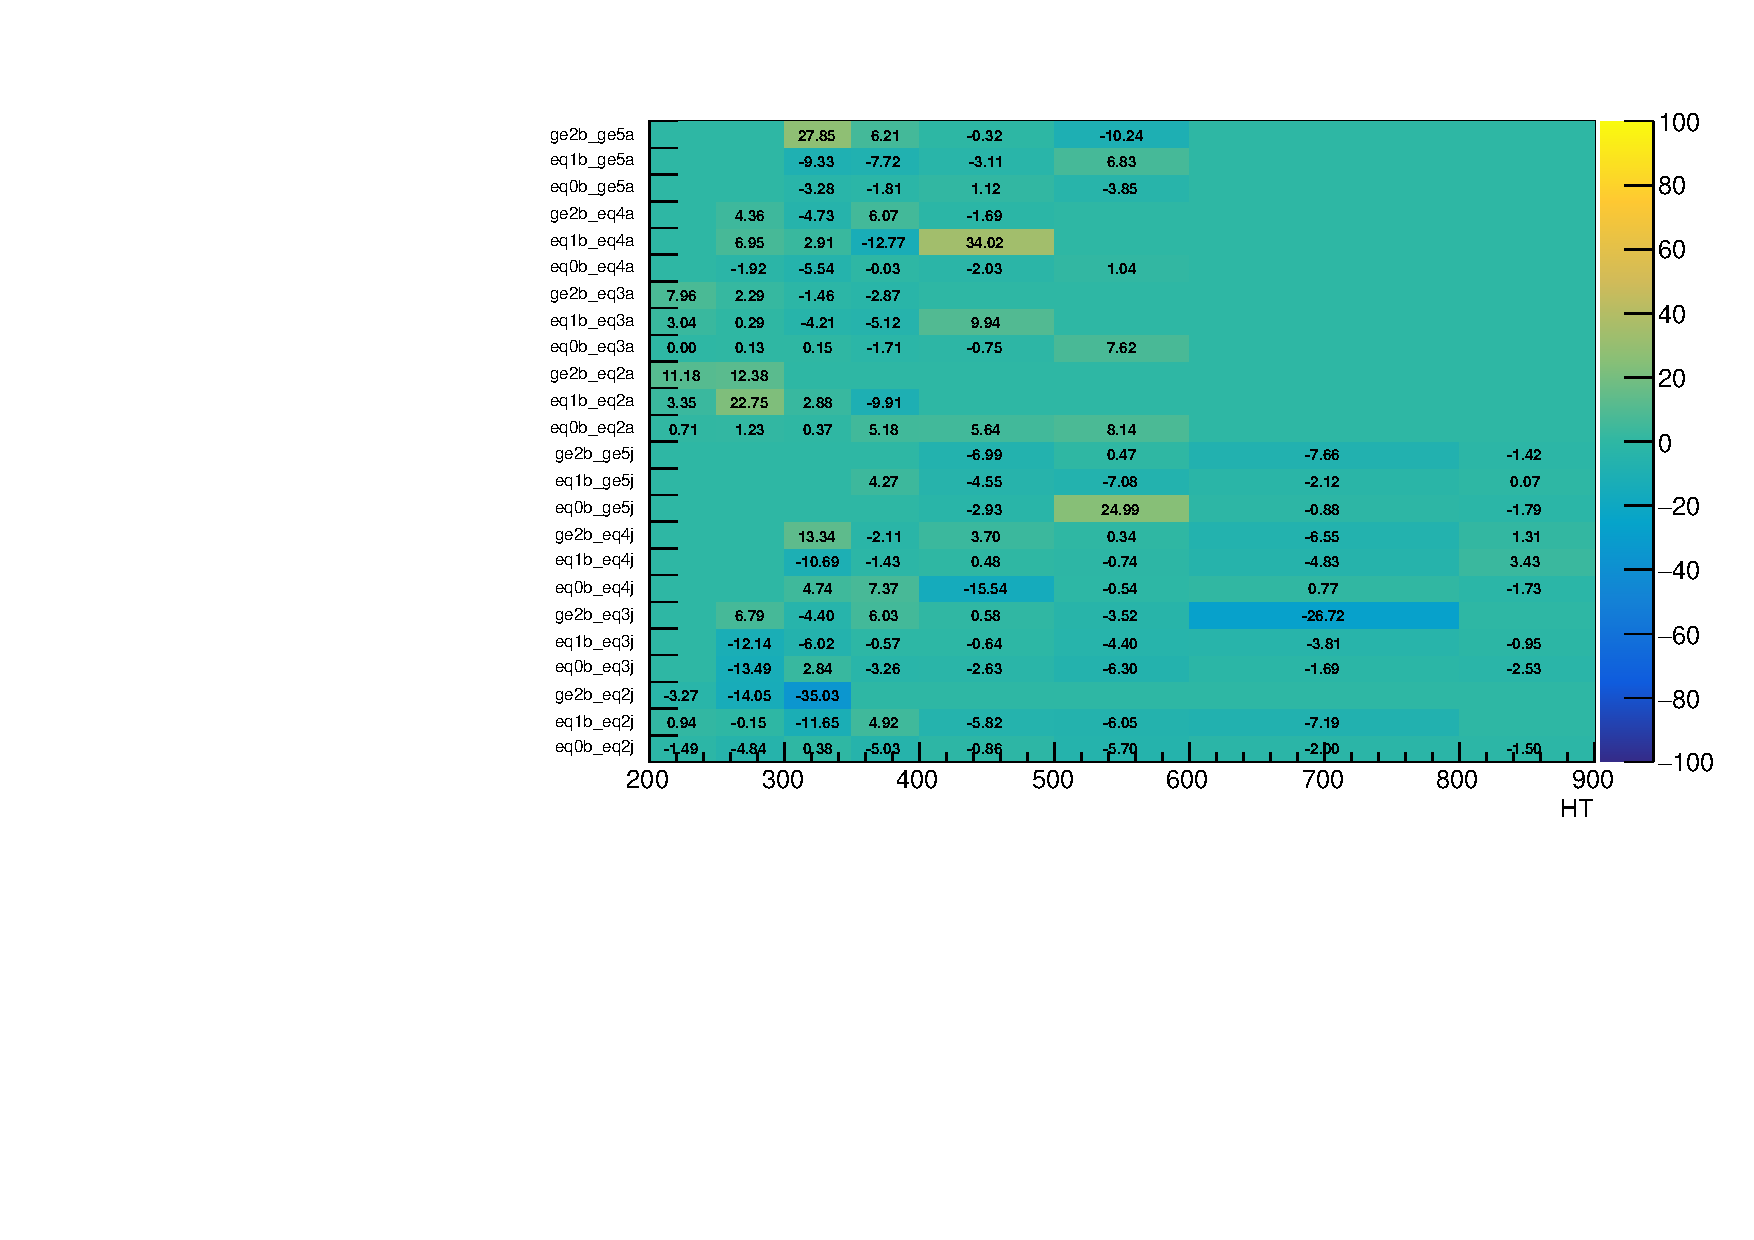
\includegraphics[width=0.55\textwidth]{figures/jesSystematics/SingleMu_MC_TF_Comp.pdf}
  } ~~
  \subfigure[The relative change in transfer factors for every
  analysis bin with an \alphat cut, inclusive on b-tags]{
    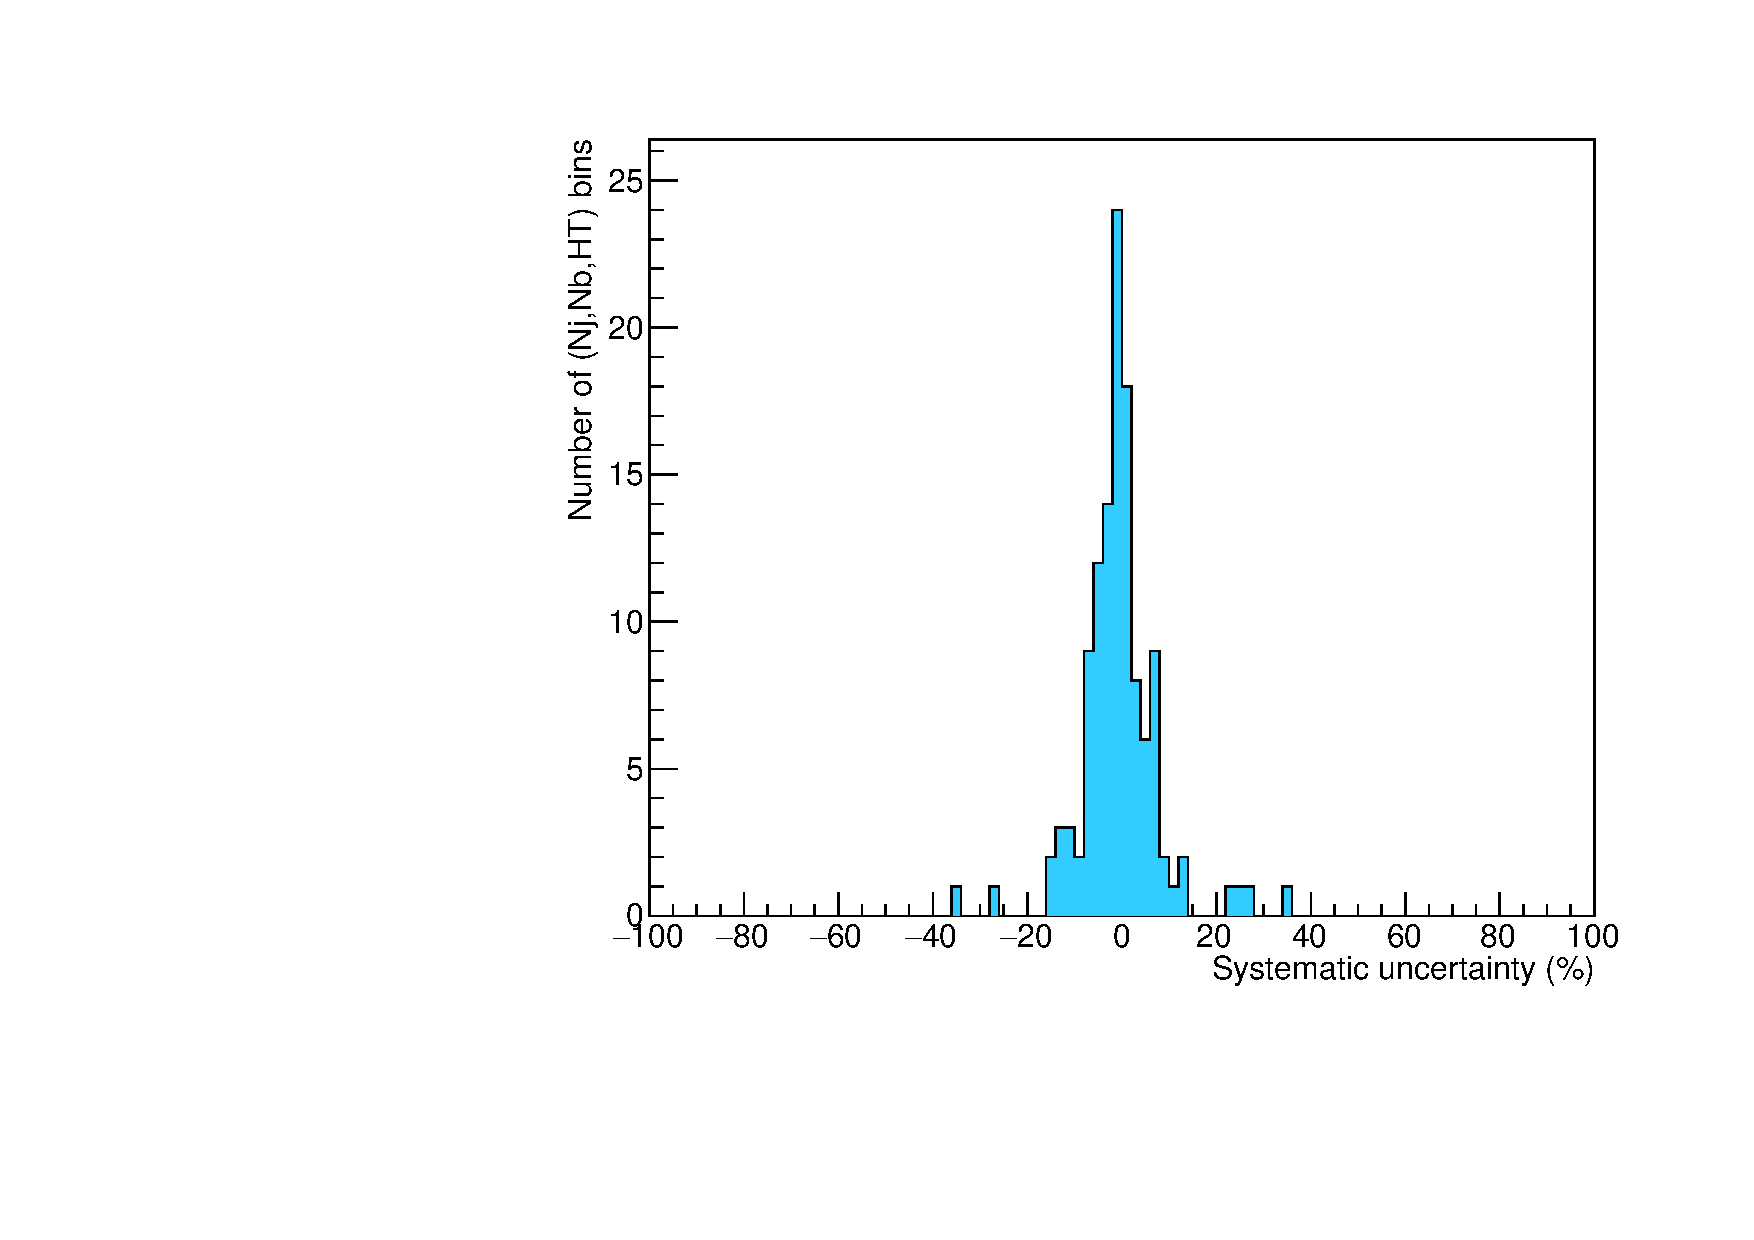
\includegraphics[width=0.44\textwidth]{figures/jesSystematics/SingleMu_MC_Systematics1D.pdf}
  }
  \caption{\label{fig:jes-syst-singleMu} The change in pseudo transfer
  factors when calculating them with nominal jet energy corrections
  and the minus one sigma level jet energy corrections in the \mj
  control sample.}
\end{figure}

\begin{figure}[]
  \centering
  \subfigure[The relative change in transfer factors per \scalht bin
  and jet category]{
    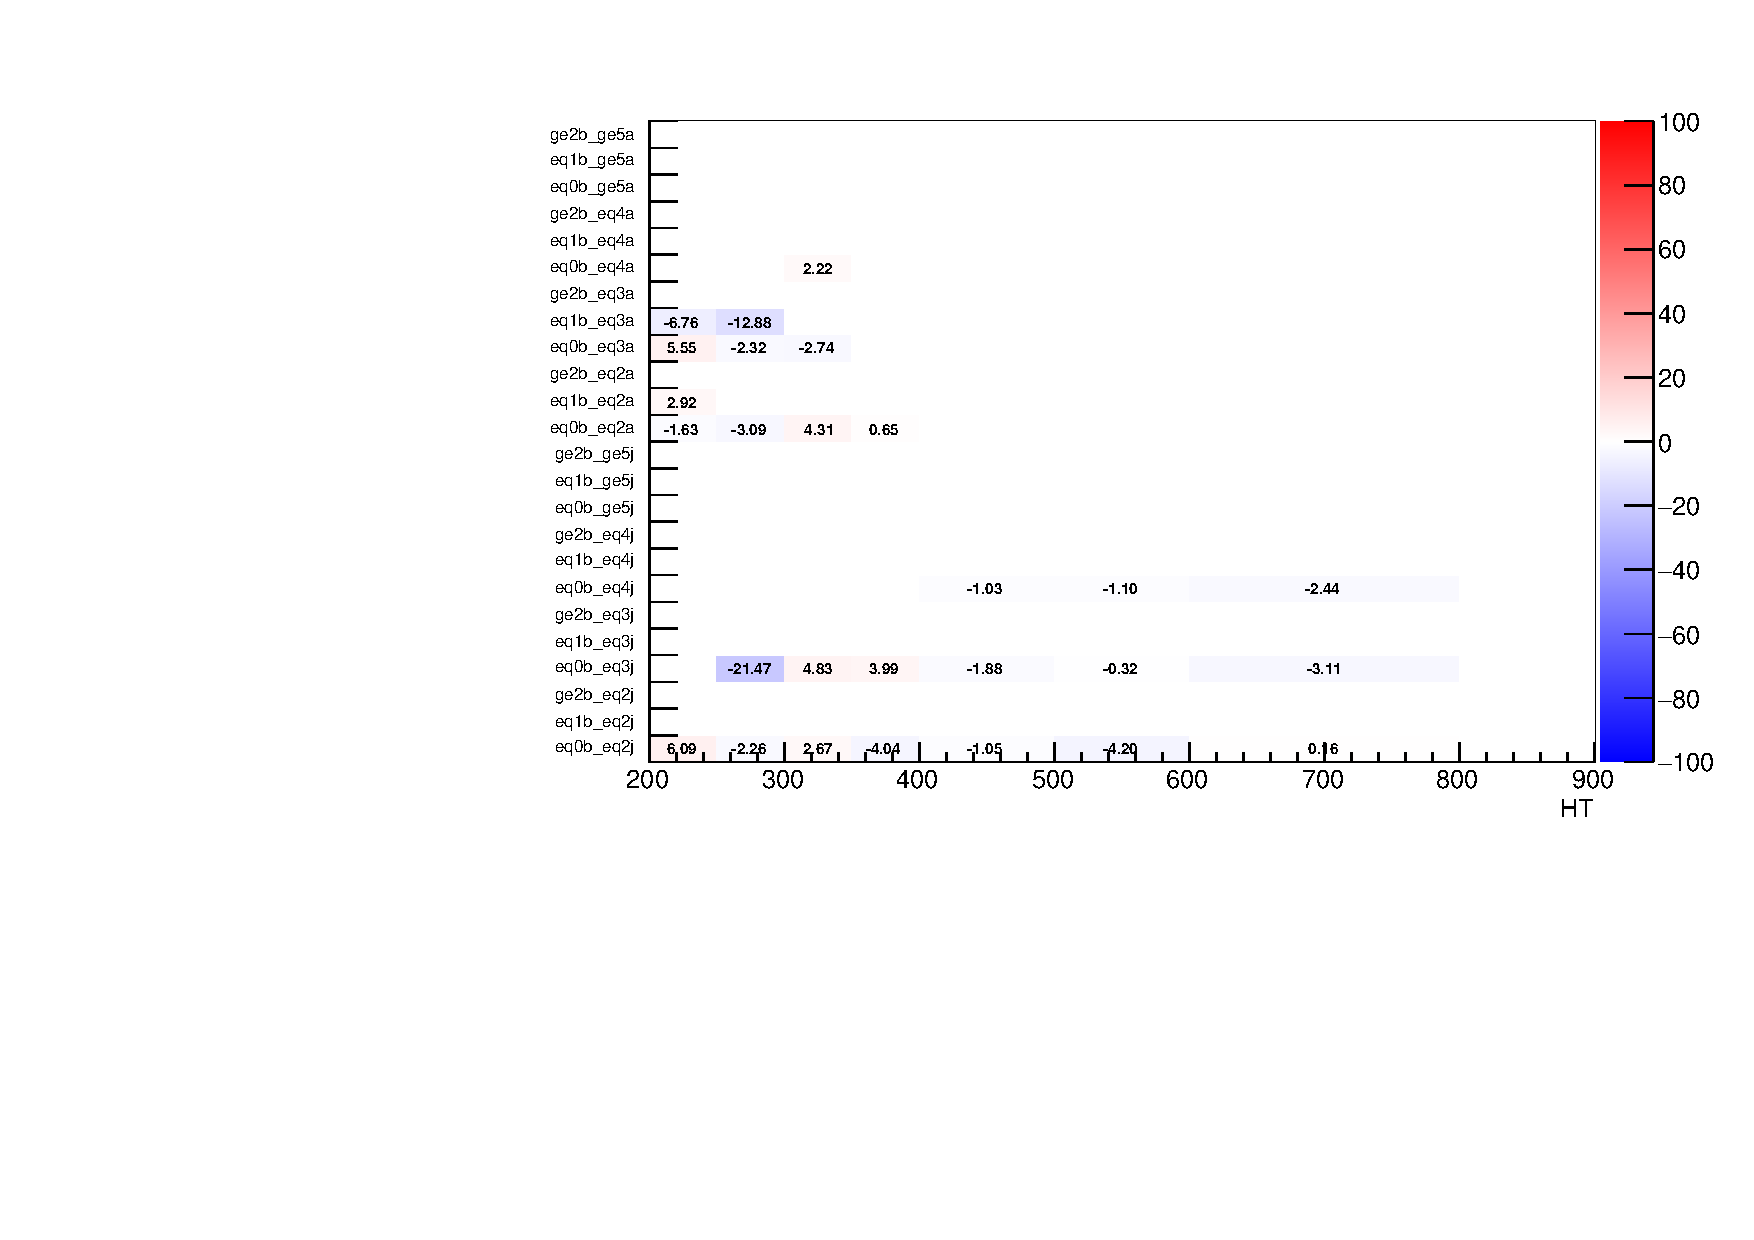
\includegraphics[width=0.55\textwidth]{figures/jesSystematics/DoubleMu_MC_TF_Comp.pdf}
  } ~~
  \subfigure[The relative change in transfer factors for every
  analysis bin with an \alphat cut, inclusive on b-tags]{
    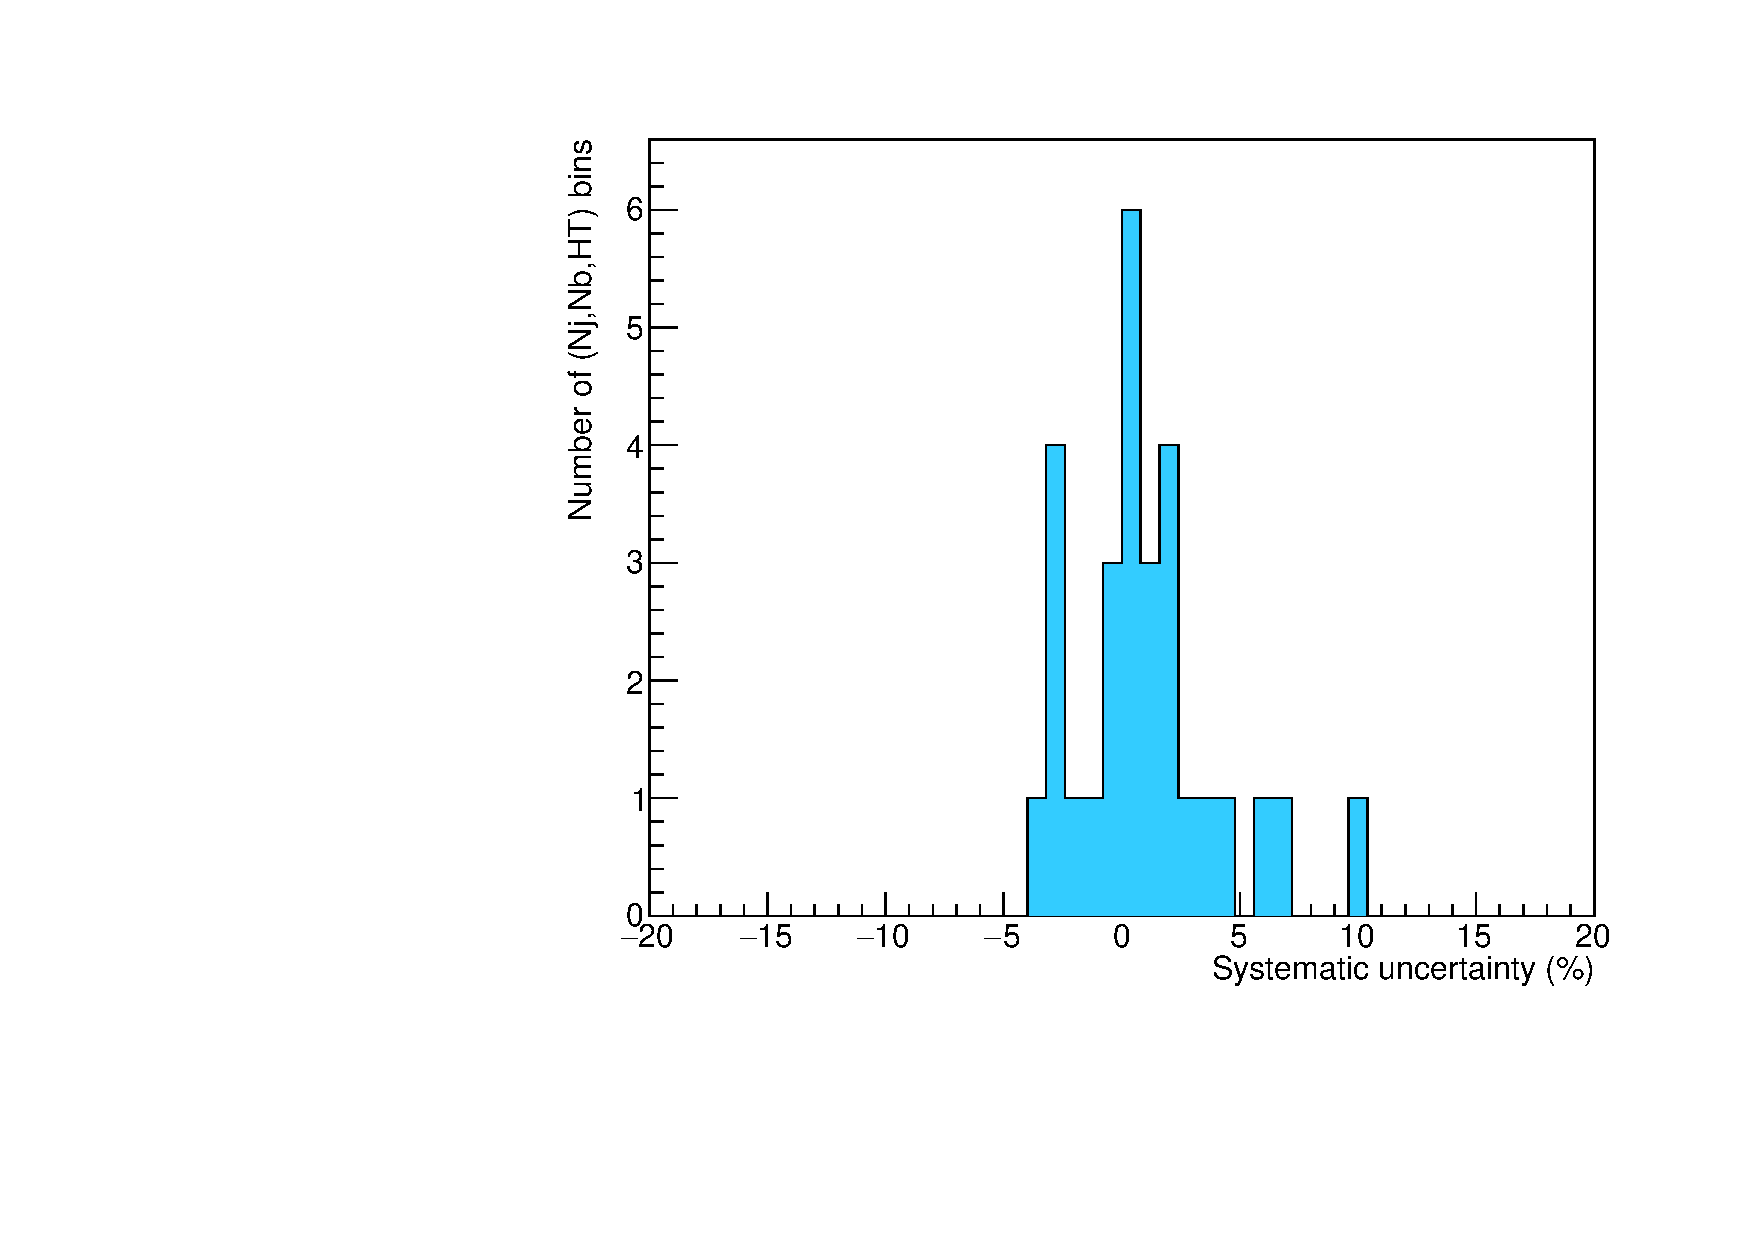
\includegraphics[width=0.45\textwidth]{figures/jesSystematics/DoubleMu_MC_Systematics1D.pdf}
  }
  \caption{\label{fig:jes-syst-doubleMu} The change in pseudo transfer
  factors when calculating them with nominal jet energy corrections
  and the minus one sigma level jet energy corrections in the \mmj
  control sample.}
\end{figure}

{\bf b-tagging efficiency scale factors}

Scale factors provided by the BTV POG are applied to the MC samples
to correct for differences in the b-tagging efficiencies and 
misidentifications between simulation and data. The method employed is
based on simple event reweighting as described in
Ref.~\cite{btagSFMethods}. Events are reweighted according to the
probability of obtaining a particular jet configuration in data
and simulation, as determined by the b-tagging efficiencies computed
in the MC samples and the scale factors measured in data.

Figure ~\ref{fig:btagSF-syst-singleMu} shows the effect on the transfer
factors in the \mj control region of varying the b-tag scale factors 
up and down by their corresponding uncertainties. The systematic
effect is very small, at the percent level or less, and is
sub-dominant with respect to the systematic errors derived from the 
closure tests.

\begin{figure}[]
  \centering
  \subfigure[]{
    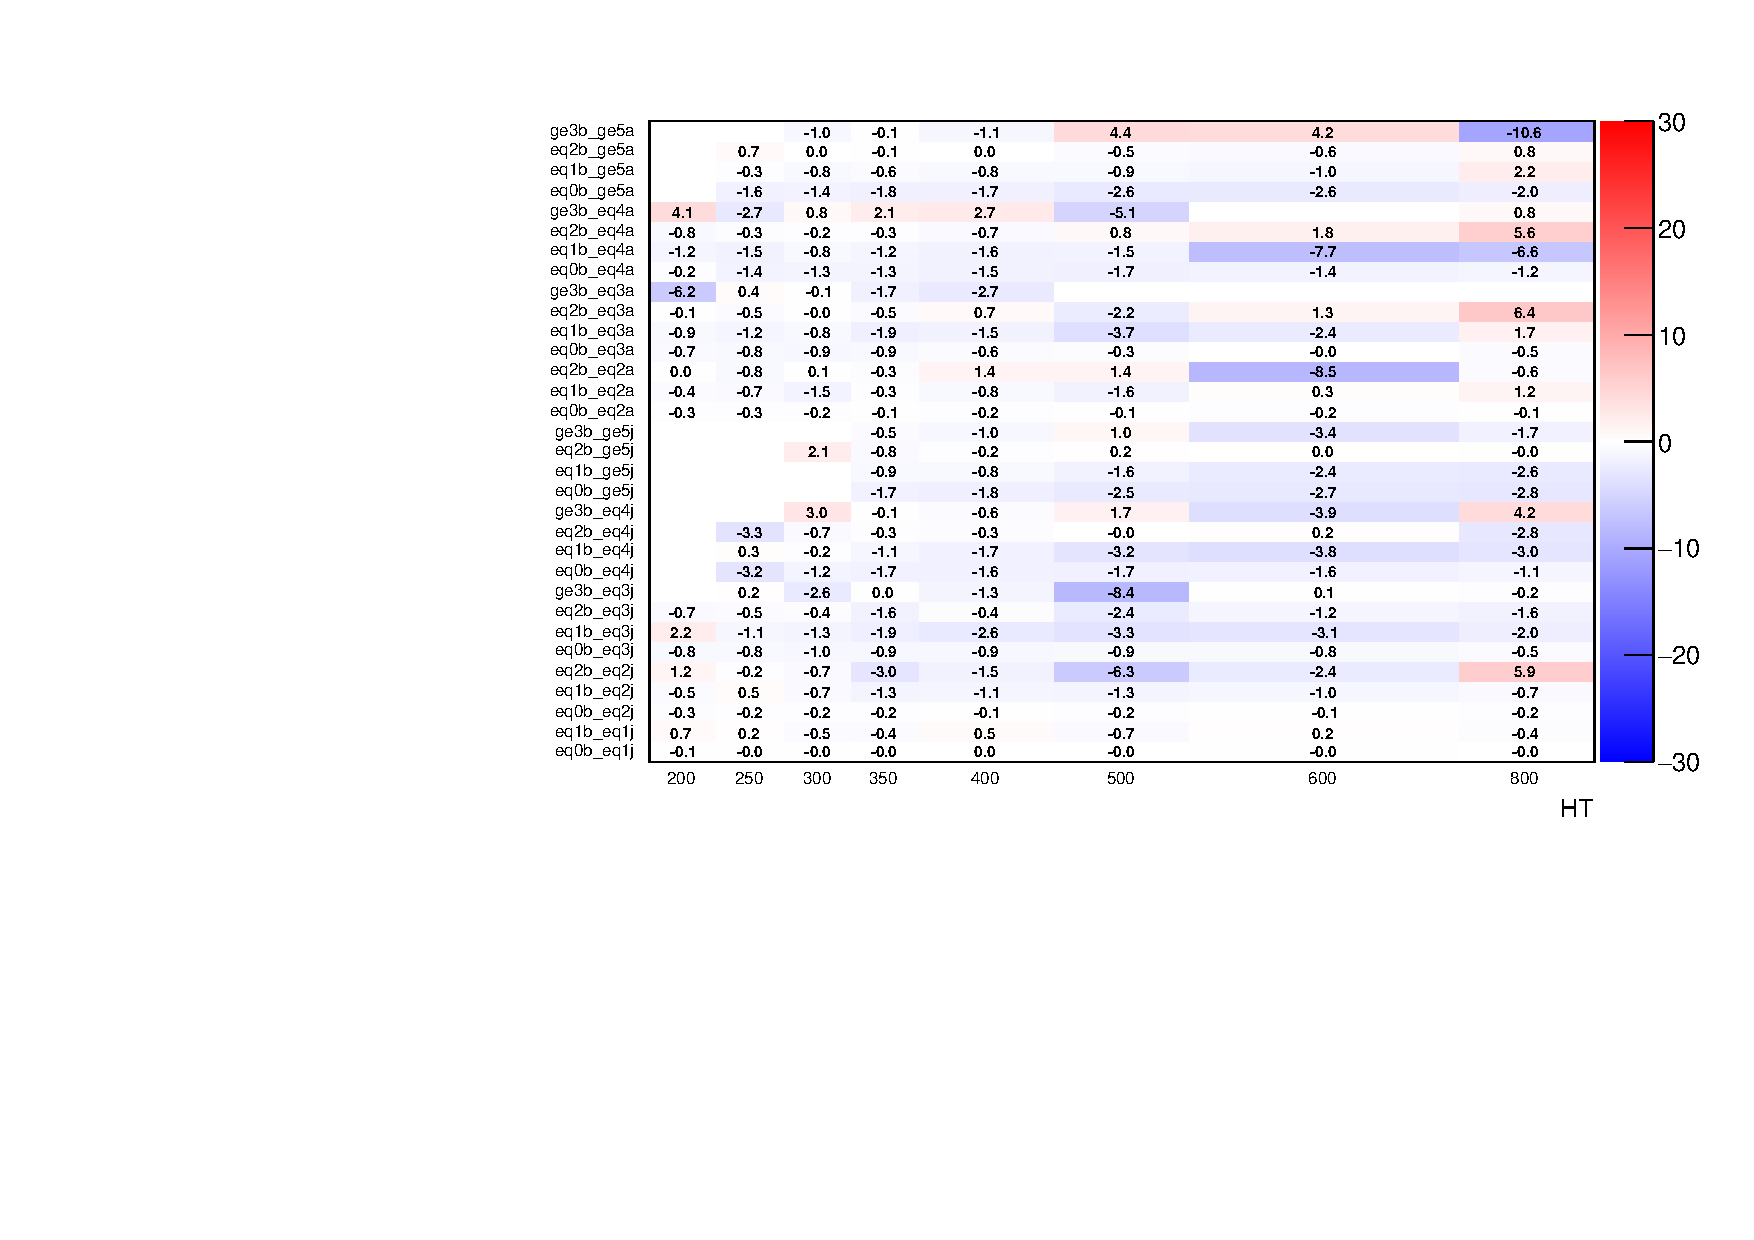
\includegraphics[width=0.5\textwidth]{figures/btagSFSystematics/Single_Muon_Ewk_Yields_SystematicDown.pdf}
  } ~~
  \subfigure[]{
    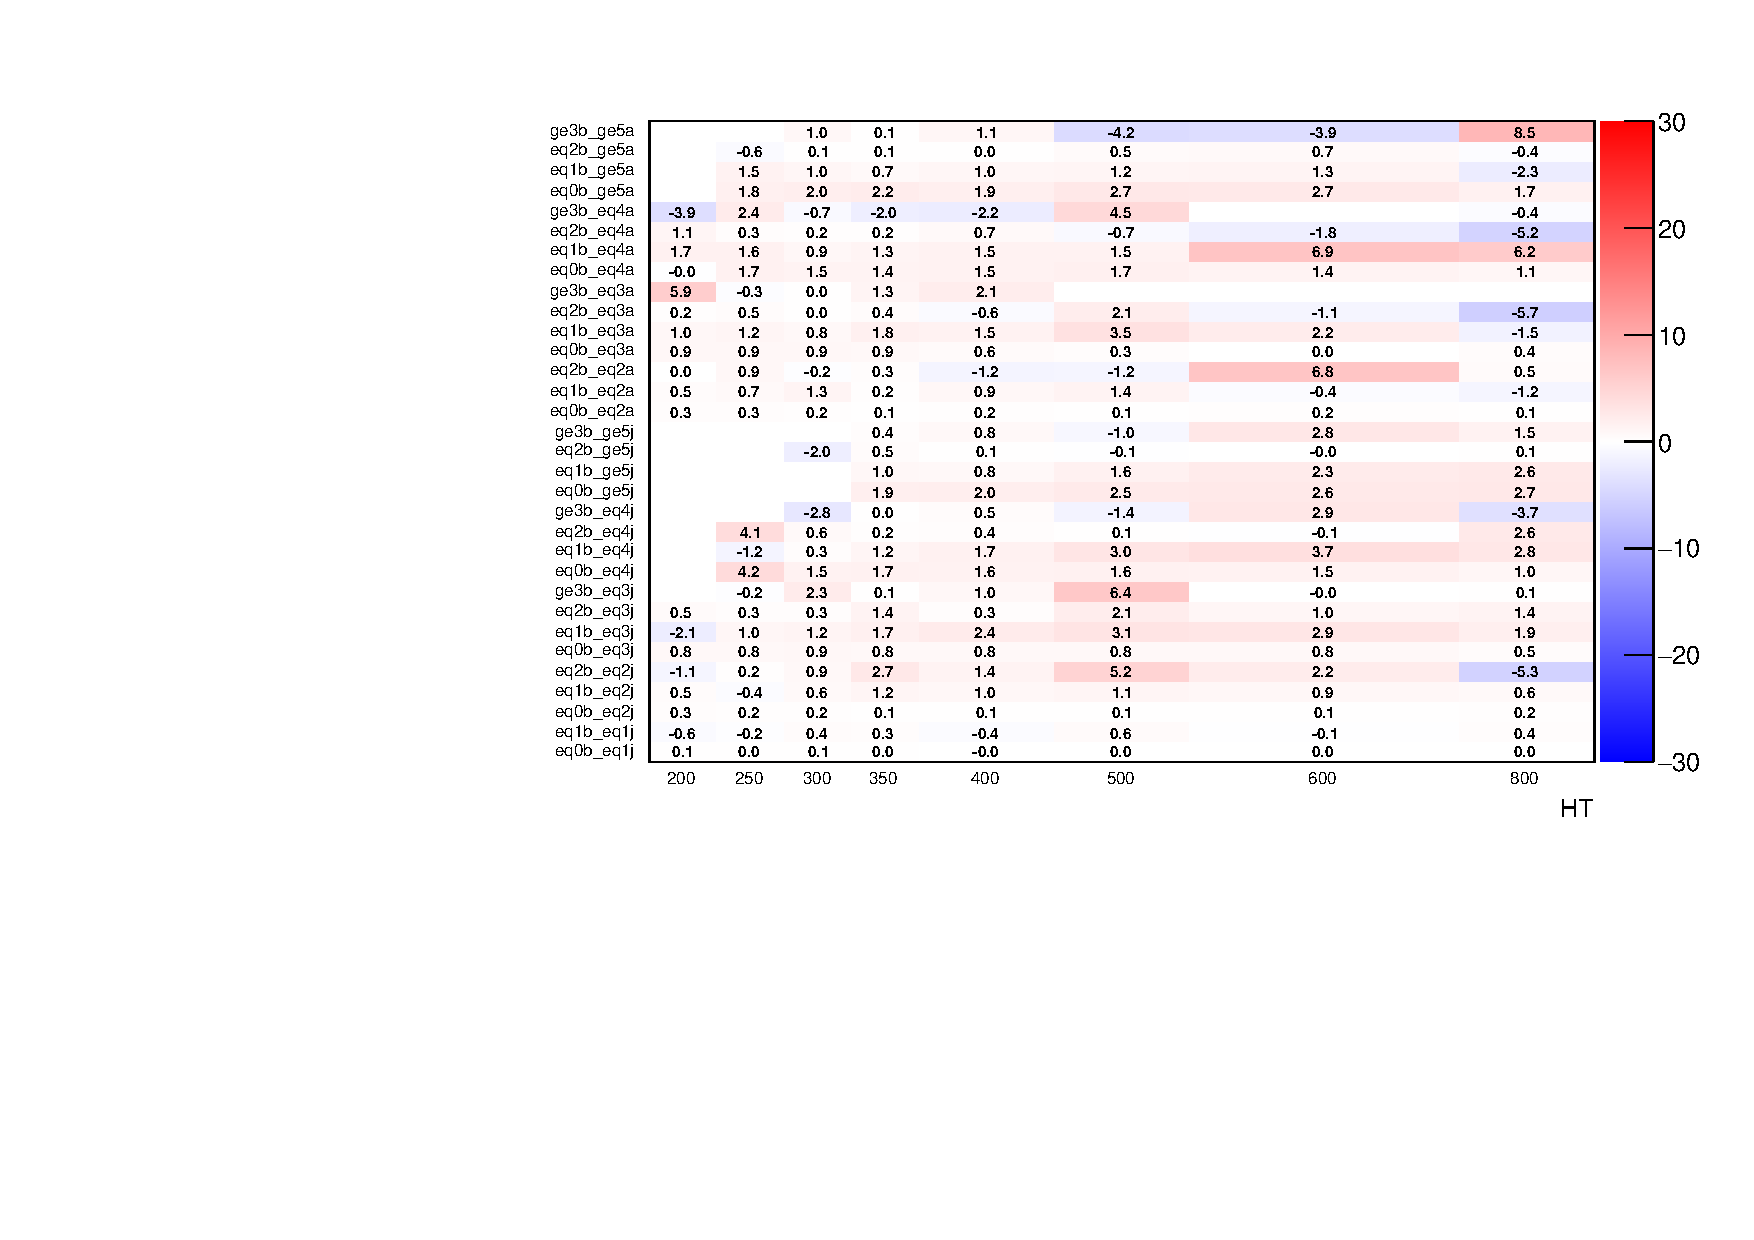
\includegraphics[width=0.5\textwidth]{figures/btagSFSystematics/Single_Muon_Ewk_Yields_SystematicUp.pdf}
  }
  \newline
  \subfigure[]{
    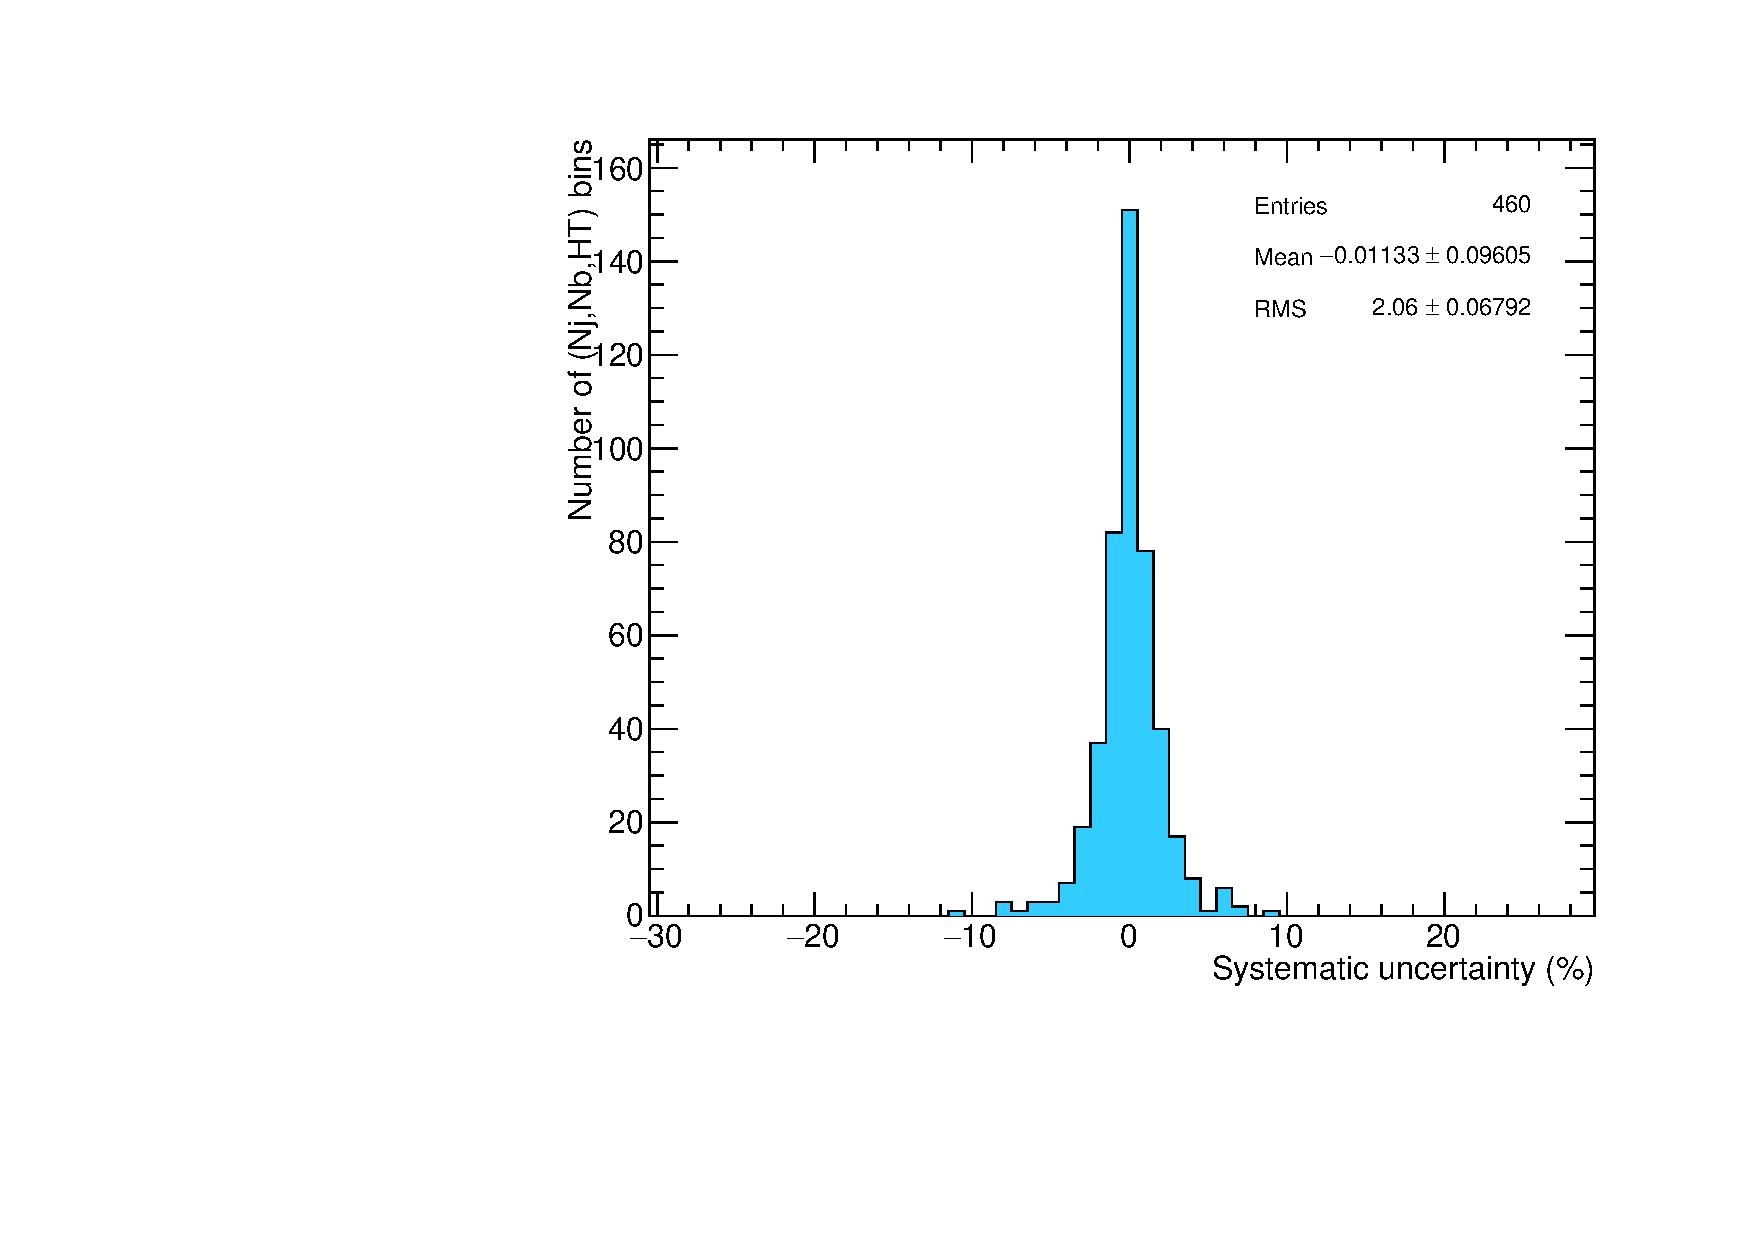
\includegraphics[width=0.5\textwidth]{figures/btagSFSystematics/Single_Muon_Systematics1D.pdf}
  }

  \caption{\label{fig:btagSF-syst-singleMu} The percentage change in
  transfer factors in the \mj control region in each
  $(\njet,\nb,\scalht)$ bin when calculating them with
  minus one sigma b-tag scale factors (a) and plus one sigma
  b-tag scale factors (b), relative to the nominal scale
  factors, as well as the one-dimensional distribution of these
  systematic changes over all bins (c), demonstrating the small effect
  of this source of systematic on the background prediction.}
\end{figure}



{\bf QCD contamination}

A check has also been performed on the systematic effect on the
background prediction due to QCD contamination in the control samples,
which has been found to be at the percent level for the \mj and \gj
control regions. Applying an arbitrarily large variation of $\pm
100\%$ on the number of Monte Carlo QCD events leads to a systematic
variation on the transfer factors of at most 5\% in the majority of
bins.

These preliminary studies suggest that the jet energy scale and QCD
uncertainties are small and should be covered by the systematics
derived from the closure tests in
Sec.~\ref{sec:closure-tests-data}. The closure tests are therefore a
conservative estimate to which it can be established, based on data,
that there is no significant bias in the background predictions. 
%A more thorough study of these and additional source of systematic
%uncertainty will be carried out in the near future. If not
%sub-dominant, these additional uncertainties will be propagated
%through to the final total.


%%%%%%%%%%%%%%%%%%%%%%%%%%%%%%%%%%%%%%%%%%%%%%%%%%%%%%%%%%%%%%%%
% Closure tests
%%%%%%%%%%%%%%%%%%%%%%%%%%%%%%%%%%%%%%%%%%%%%%%%%%%%%%%%%%%%%%%%

\subsection{Data driven systematics with closure tests}
\subsubsection{Definition of a closure test}
\label{sec:closure-tests-desc}
\label{sec:bkgdnorm-syst}

The background estimates determined in each (\njet,~\nb,~\scalht) bin
rely on transfer factors to extrapolate data counts in control region
bins to predictions in the corresponding signal region bins, as
described in Sec.~\ref{sec:ewk-method}. Since the transfer factors are
obtained from simulation, an appropriate systematic uncertainty is
assigned to each transfer factor to account for limitations in the
simulation modelling of event kinematics and instrumental effects. The
next sections describe how the systematic uncertainties are determined
from closure tests in data.

The sensitivity of the transfer factors to potential limitations in
the simulation modelling is established through sets of closure tests,
which confront data yields measured in one data control (sub-)sample
against the predictions determined from another data control
(sub-)sample as a function of \scalht. \ie, an extrapolation is made
from one control (sub-)sample to another (rather than to the signal
region) in bins of \scalht via transfer factors determined from
simulation. A large ensemble (\ie hundreds) of closure tests are
performed between a number of control (sub-)samples to identify any
potential sources of bias in the transfer factors.

The level of statistical consistency between the predicted and
observed yields of each closure test in the ensemble is inspected. The
level of agreement between the predicted and observed yields is
expressed as the ratio $(\nobs - \npre)/\npre$ while considering only
the statistical uncertainties on \npre and \nobs. Therefore, the level
of closure is defined by the statistical significance of a deviation
in the ratio from zero. A ``set'' of closure tests includes
statistically independent tests determined as a function of \scalht
(according to the \scalht binning used in the control and signal
regions). In this way, a set of closure tests allows one to establish
the presence of significant biases or dependence on
\scalht. Importantly, if statistically significant biases are
observed, further studies are required to understand and correct for
these biases. %The metrics used to determine \fixme{HERE!!!!!!!!}. 

Under the assumption of closure for each test of the ensemble,
systematic uncertainties on the transfer factors are derived for each
(\njet,~\nb) category and \scalht bin. The treatment for estimating
the systematic uncertainties on the transfer factors is described in
Sec.~\ref{sec:syst-from-closure}.

The closure tests rely on the \mj, \mmj, and \gj control samples,
as defined in Secs.~\ref{subsec:mucontrolSelection},
\ref{subsec:mumucontrolSelection}, and
\ref{subsec:photoncontrolSelection}. (The \ej and \eej control samples
are not currently used.)

The following closure tests are not the only ones considered or
checked, \ie, the list above is not exhaustive. However, they are a
representative set that cover the main potential sources of bias in
the transfer factors derived from simulation. 

\subsubsection{Systematic uncertainties from closure tests\label{sec:syst-from-closure}}

Each set of closure tests should demonstrate in data, within the
statistical precision of each test, that there are no significant
biases or dependencies on \njet nor \scalht inherent in the transfer
factors obtained from simulation. 
Once it is established that no significant bias or trend is observed
for any set of closure tests, the systematic uncertainties associated
with the transfer factors are determined from ensembles of closure
tests. The statistical precision of the closure tests are considered
when determining the systematic uncertainties that are assigned to the
transfer factors, as it is only the statistical uncertainties
associated with the tests that limit our knowledge of whether closure
is actually achieved or otherwise. Ensembles comprising several tests
are considered in bins of (\njet,\scalht) to derive a systematic
uncertainty for that bin. 

The systematic uncertainties in the transfer factors are considered as
a ``normalisation'' uncertainty in the SM background predictions,
which are determined per (\njet,~\nb) category per \scalht bin and are
assumed to be fully uncorrelated between the different (\njet,~\nb)
categories and \scalht bins. Further details or the likelihood model
are provided in Section \ref{sec:likelihood}. The systematic
uncertainty is estimated by taking the quadrature sum of the weighted
mean and (square root of) weighted sample variance for the closure
tests within the given \scalht bin.

In order to find ``expected systematics'', \nobs and \npre are
determined from the same sample of simulated events (that guarantees
closure) with statistical uncertainties errors are taken from the
unweighted and weighted counts, respectively. The expected systematic
uncertainty is then taken as the weighted mean of the error on the
ensemble of closure tests. This is an estimator of the expected
variance, assuming no bias is found in data.

We note the behaviour of the magnitude of the systematic uncertainties
on the integrated luminosity, which reduce with increasing
luminosity. This is a reflection of the fully statistical nature of
the ``systematic'' in the absence of bias.

Several versions of this search have derived a single set of
process-independent systematic uncertainties as a function of
(\njet,~\nb,~\scalht) based on a single ensemble of a core set of
closure tests. 

During the Early Analysis review, an alternative approach was advised,
which involves splitting the closure tests into different ensembles,
each specific to a particular process or effect and containing only
the most relevant closure tests. This allows for the independent
derivation of systematic errors that is specific to a background
process.

\subsubsection{Tests probing the prediction of the \znunu
background with the \mmj control sample}

Closure tests that probe the modelling of the \alphat and
\bdphi extrapolations in the analysis are also performed. In both
cases, the test checks if events with genuine \met found in the core
of the variable distribution below some threshold value can be used to
predict the events in the tail (above the same threshold value). 

The closure tests in Fig.~\ref{fig:closureAlphaT} probe the modelling
of the \alphat distribution (following the application of the $\mht >
130\gev$ requirement in the control and signal regions) in genuine
\met events as a function of \scalht. This is important to verify the
approach of using \mj and \mmj samples without an \alphat requirement
to make background predictions in the signal region. The tests
confront data yields in a \mj (\mmj) samples with an \alphat
requirement against predictions determined in a \mj (\mmj) sample with
the \alphat requirement inverted. As usual, corresponding expectations
from simulation are obtained to construct the transfer factors
required to make the predictions.

These closure tests are not considered in the ensembles presented in
Sec.~\ref{sec:closure-tests-data} (as was normally the case for
previous iterations of the analysis) and instead added as a new
separate ensemble from which an additional contribution to the total
systematic uncertainty per (\njet,~\nb,~\scalht) bin is derived. These
contributions are assumed be be fully correlated across \nb (and
uncorrelated as a function of \njet and \scalht). The magnitude of
these contributions are presented in Table~\ref{tab:alphaTSyst}. For
$\scalht<800\gev$ these numbers are derived from the \alphat closure
tests. However, as there is no \alphat requirement for
$\scalht>800\gev$, the $\Delta\phi *$ closure tests in
Sec.~\ref{sec:closureCrossCheck} are used to derive the systematic in
this case.

\begin{figure}[h!]
  \begin{center}
    \subfigure[]{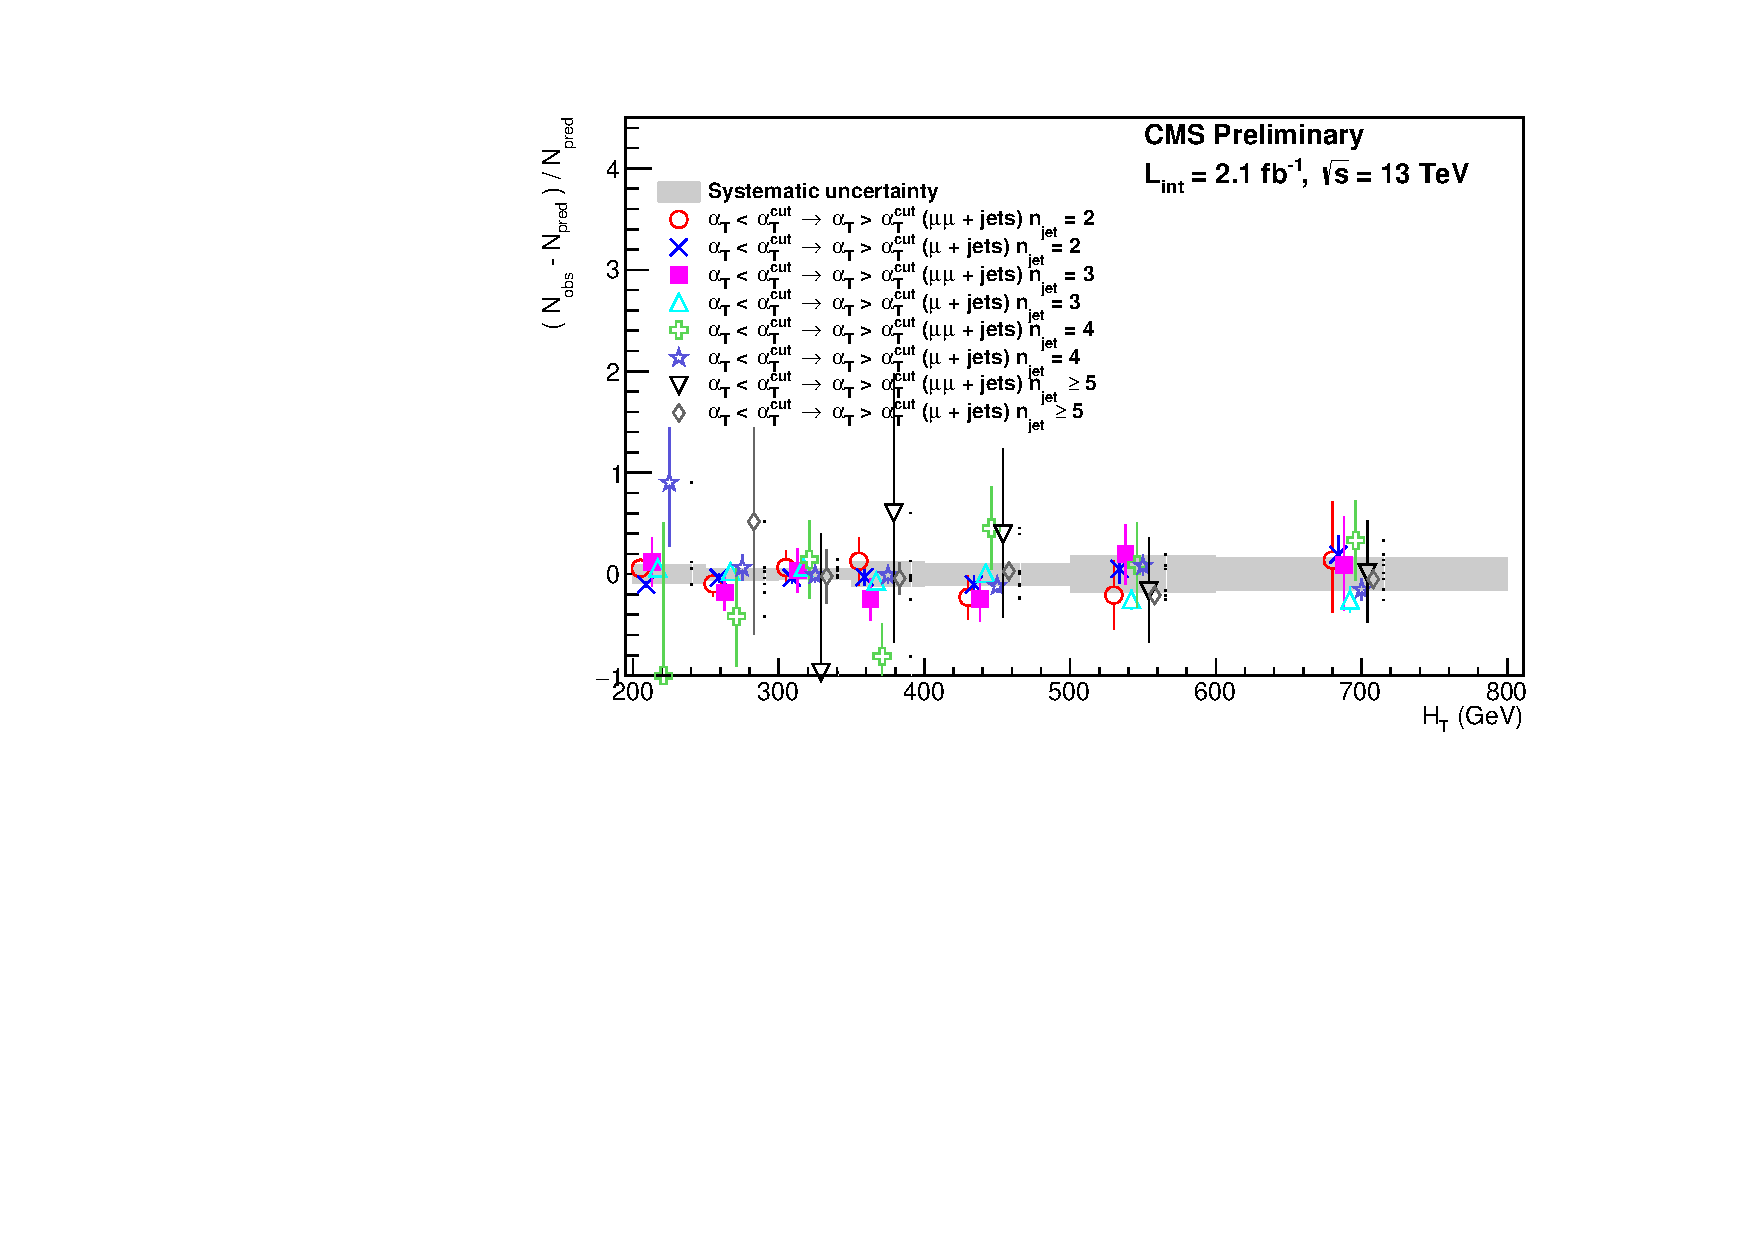
\includegraphics[width=0.6\textwidth]{figures/closureTests/newJamboree/alphaTOnlyTest.pdf}}
    ~~
    \subfigure[]{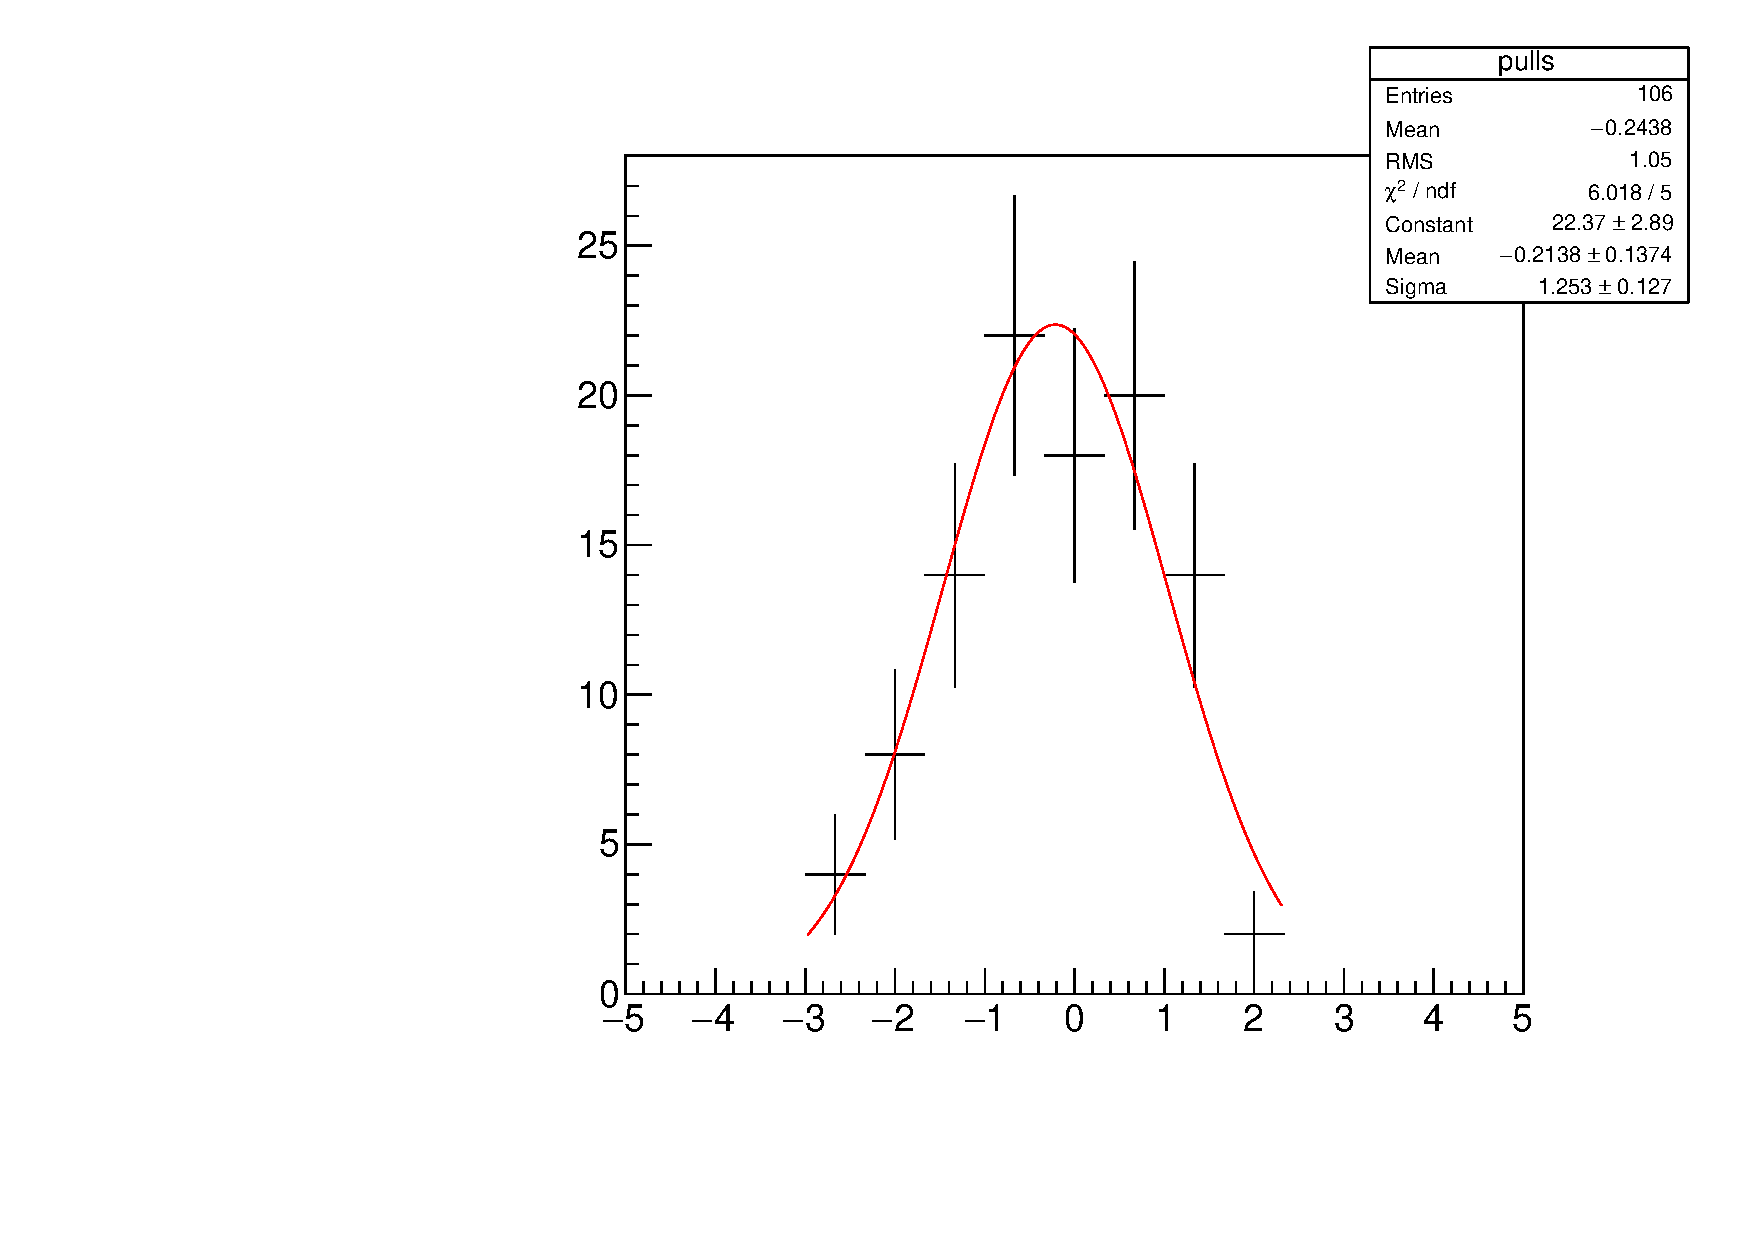
\includegraphics[width=0.4\textwidth]{figures/closureTests/newJamboree/alphaTPulls.pdf}} 
    \caption{Closure tests probing the \alphat extrapolation for each
      \njet category (open symbols) overlaid on top of the systematic
      uncertainty estimates used for each of the seven \scalht bins
      (shaded bands) carried out with $2.1\ifb$ of $13\tev$
      data. Also shown are the pulls for each closure test.}
    \label{fig:closureAlphaT}
  \end{center} 
\end{figure}

\begin{table}[h!]
  \caption{Systematic uncertainties (percent) in the
    predictions of the $\ttbar$W and $\znunu$ (the latter in
    parentheses) background components as a function of \scalht due to
    the extrapolation in the \alphat (\bdphi) variable in the region
    $\scalht > 800\gev$ ($\scalht > 800\gev$), as determined from
    ensembles of closure tests in multiple data control samples. The
    data control samples correspond to an integrated luminosity of
    2.1\fbinv.} 
  \label{tab:alphaTSyst}
  \centering
  \footnotesize
  \begin{tabular}{ cccccccc }
    \hline
    \hline
    \multicolumn{8}{c}{\scalht bin (GeV)}                                       \\
    \hline
    200   & 250     & 300     & 350     & 400     & 500     & 600     & 800     \\
    10 (10) & 7 (7) & 8 (8) & 17 (17) & 14 (14) & 24 (24) & 27 (27) & 22 (22) \\
    \hline
    \hline
  \end{tabular}
\end{table}

The closure tests in Fig.~\ref{fig:closureBDPhi} probe the modelling
of the $\Delta\phi *$ distribution in genuine \met events as a
function of \scalht. This is important to verify the approach of using
\mj and \mmj samples without an $\Delta\phi *$ requirement to make
background predictions in the signal region. The tests confront data
yields in a \mj (\mmj) samples with an $\Delta\phi *$ requirement
against predictions determined in a \mj (\mmj) sample with the
$\Delta\phi *$ requirement inverted. 

\begin{figure}[h!]
  \begin{center}
    \subfigure[Closure
    tests]{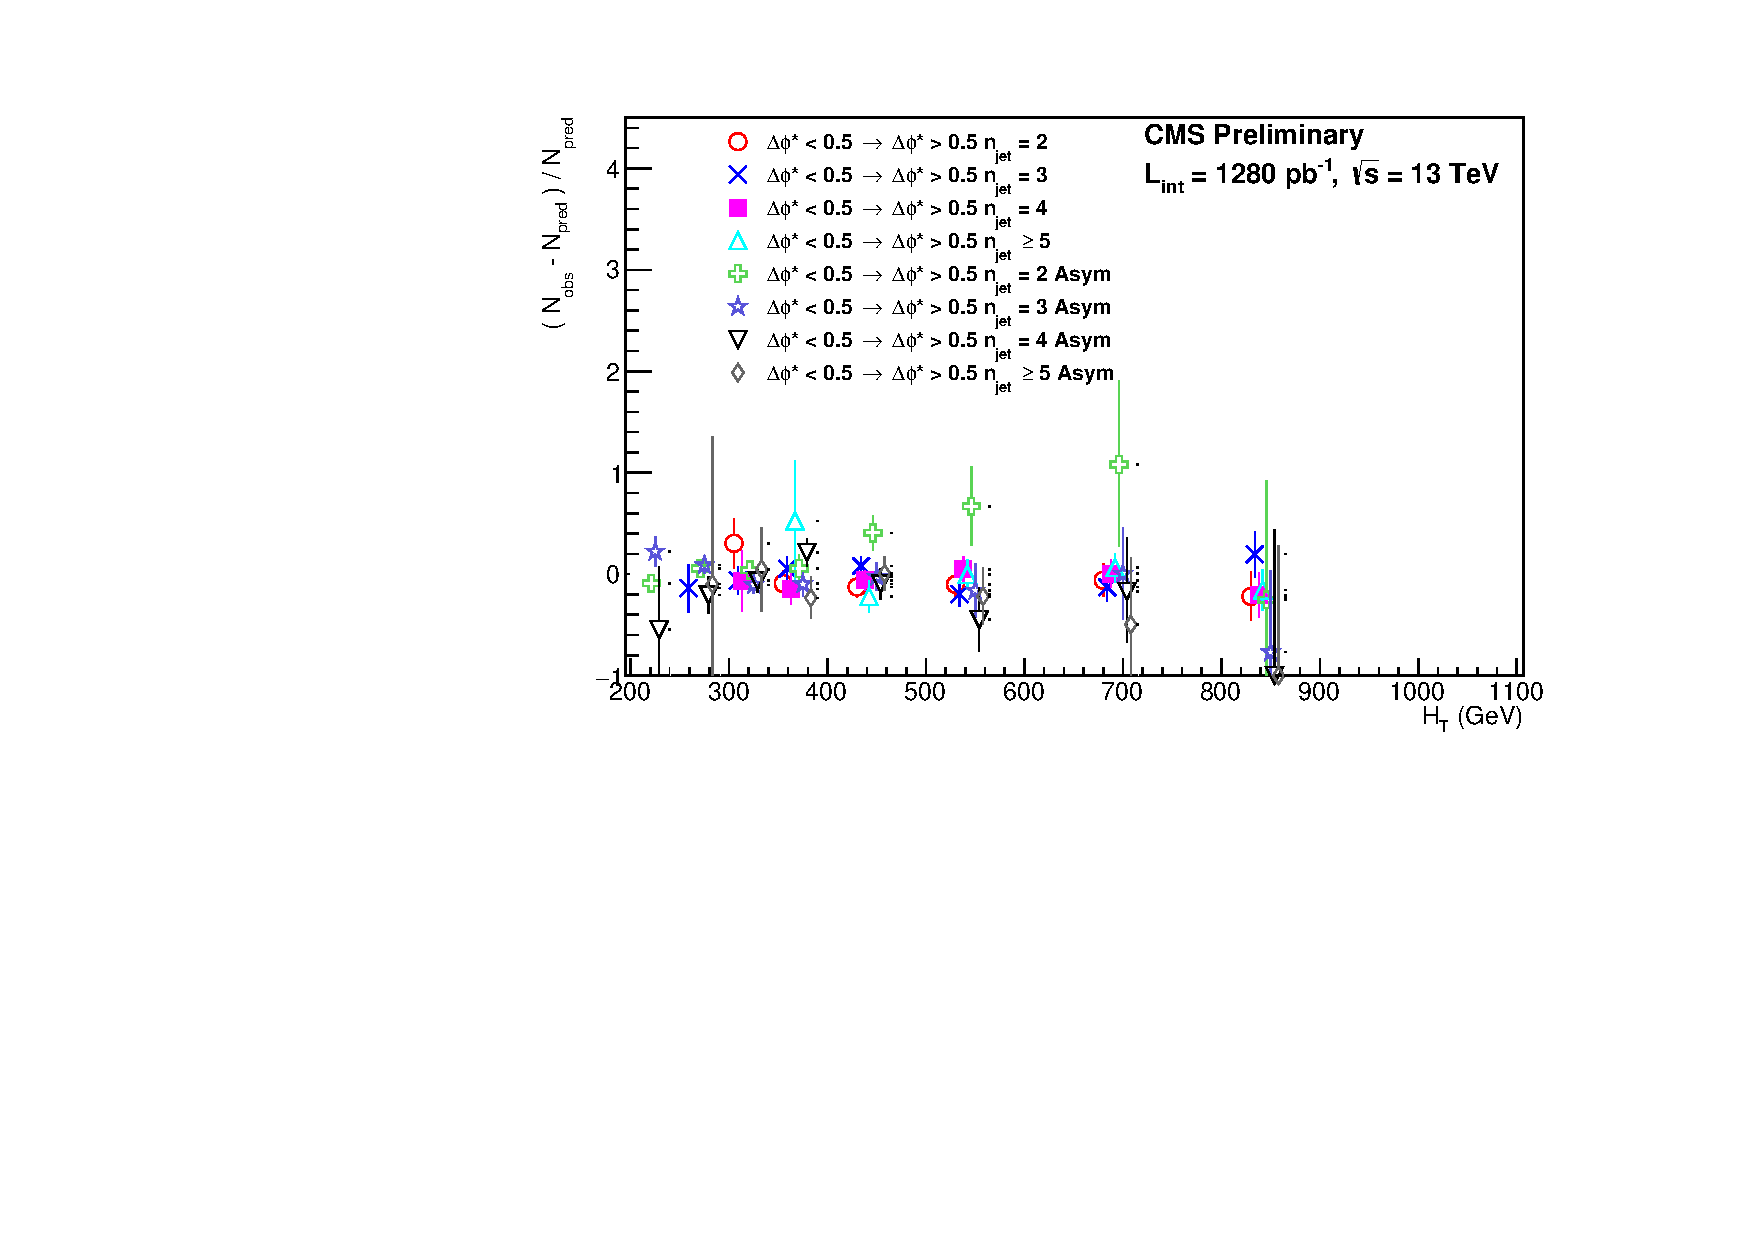
\includegraphics[width=0.6\textwidth]{figures/closureTests/newJamboree/bDPhiCrossCheck.pdf}}
    ~~
    \subfigure[Pulls of closure
    tests]{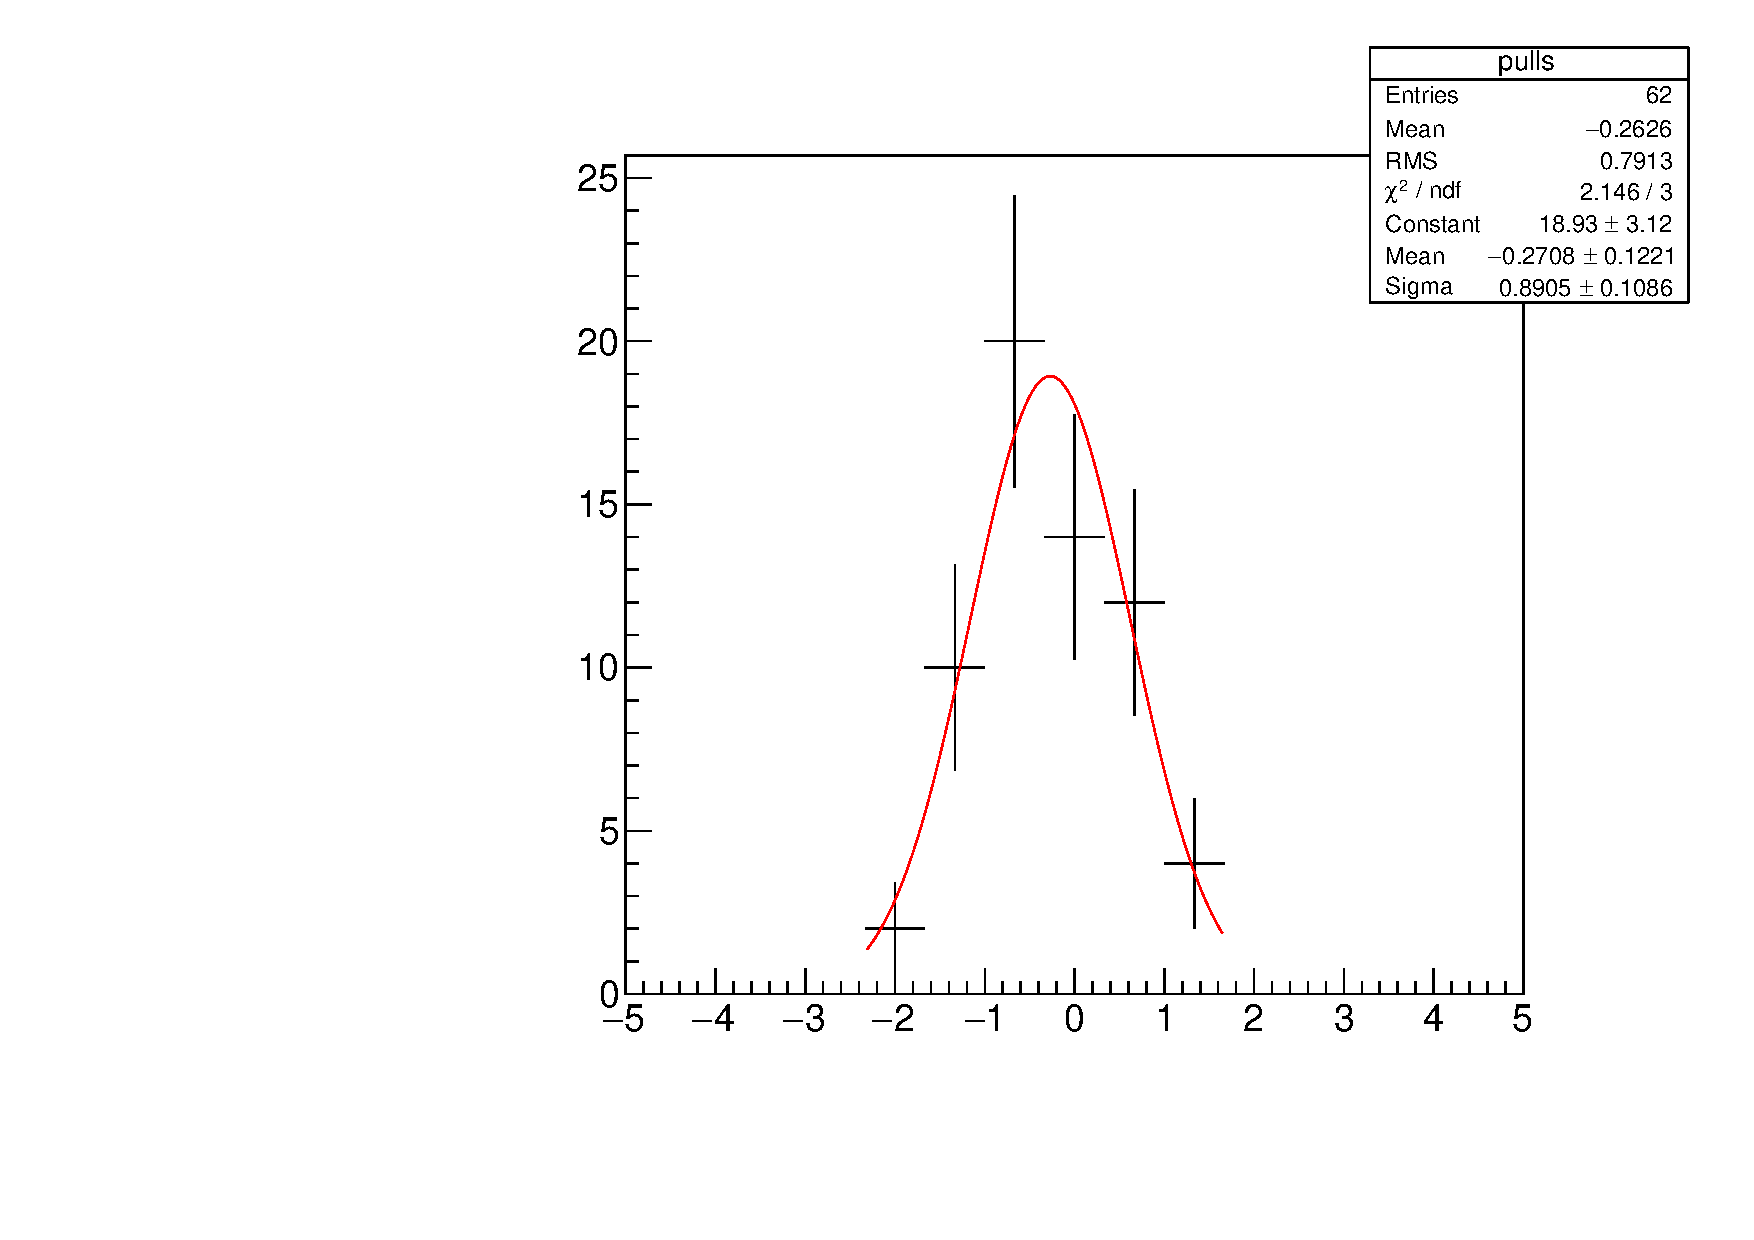
\includegraphics[width=0.4\textwidth]{figures/closureTests/newJamboree/bDPhiPulls.pdf}} 
    \caption{Closure tests probing the $\Delta\phi *$ extrapolation for each
    \njet category (open symbols) and their pulls fit with a gaussian.
    Made with the \mj control sample, carried out with $2.1\ifb$ of
      $13\tev$ data. }
    \label{fig:closureBDPhi}
  \end{center} 
\end{figure}

\subsubsection{Tests probing the prediction of the \znunu
background with the \mj control sample}

The $\mj \rightarrow \mmj$ tests deal with the consistency
of the prediction of \wej with $\gamma$ + jets, even in the presence
of contamination from \ttbar. This is important for understanding the
consistency of the \znunu + jets background prediction from \wej
events along with the associated assumptions.

Additionally, to test the prediction of \znunu + jets processes with
the $W$-enriched \mj control sample, we introduce the
$\mu^{+}\rightarrow\mu^{-}$ closure test, as mentioned in
Sec.~\ref{sec:backgroundmet}. The production mechanism of $W$ from pp
collisions means high $p_T$ $W$ bosons are predominantly left handed
\cite{WPol}.  For high $p_T$ bosons, this implies that $W^+$ decays to
the left handed neutrino along its direction of motion while the
lepton is pointing backward. The opposite behaviour is expected for
the $W^-$. The lepton is therefore more boosted (and the neutrino less
boosted) in $W^+$ decays than $W^-$ decays.  This leads to a larger
number of $W^+$ decays in the single lepton control regions (which
relies on the lepton $p_T$ for acceptance) than in the signal region
(which relies on the neutrino $p_T$ for acceptance). The new closure
test checks if this leads to a bias in the prediction of the \znunu +
jets background. 


\subsubsection{Tests probing the prediction of the \znunu
background with the \gj control sample}

The $\gj \rightarrow \mmj$ tests deal with the
consistency between the \zee + jets and $\gamma$ + jets samples, which
is a further check on the validity of using the \gj process to predict
the \znunu\, + jets process. The muon trigger and reconstruction
efficiencies are also indirectly probed, given that different numbers
of muons are required in each of the two sub-samples.
%However, dedicated data-driven methods are used to measure the muon
%trigger and reconstruction efficiencies, with values taken from the
%muon POG.

The control of the \znunu\ + jets background, established via the
tests described above, is also validated with the full Run~1 data set
at $\sqrt{s} = 8\tev$, as described in
Appendix~\ref{app:zInvBgControl}.

\subsubsection{Tests probing the prediction of the W and \ttbar
backgrounds with the \mj control sample}

The $0$ b-tag $\rightarrow1$ b-tag
tests probe the sensitivity of the transfer factors to the relative
admixture of events from the $W$ + jets and \ttbar processes by
varying the number of b-tagged jets within the \mj sample. These tests
are conservative, as the admixture changes little between the \mj
sample and the signal region (as there is no extrapolation in \nb),
whereas the closure tests use sub-samples with different \nb bins and
therefore different admixtures of $W$ + jets and \ttbar events. \eg,
the former uses a $W$-enriched sub-sample (selected by requiring zero
b-jets) to predict yields in a \ttbar-enriched sub-sample (selected by
requiring one b-jet).

The aforementioned two b-tag related tests also probe the modelling of
the reconstruction of b-quark jets, although this is addressed more
precisely by dedicated studies involving varying the uncertainties in
b-tag scale factors, as the one performed in the previous analysis,
see for instance \cite{CMS_AN_2013-366}. Until the formula method is
applied, the b-tag SFs will be applied and their uncertainties
propagated through to the transfer factors. These variations will be
taken as an additional contribution to the total normalisation
systematic uncertainties per (\njet,~\nb,~\scalht) bin. However, based
on the behaviour observed during Run~1, these are a sub-dominant
contribution to the total systematic uncertainties.

The $\mu^{+}\rightarrow\mu^{-}$ is also employed here to ensure there
any asymmetries introduced from W polarisation effects are covered by
an appropriate systematic.


\subsection{Summary of normalisation systematic uncertainties based on $2.1~\ifb$}
\label{sec:closure-test-syst}

%%%%%%%% FIXME PUT IN CLOSURE TEST MATPLOTLIB PLOTS AS WELL

Normalisation systematics are derived from the closure test ensembles,
described above, based on the current data set, which are summarised
in Table~\ref{tab:systs}. In the kinematically restricted bins, such
as those with a high jet multiplicity and low value of \scalht, the
limited statistics leads to large systematic errors. These bins are
not used in the analysis. 
%As a minimum number of events is required for each bin considered in
%the final stages of the analysis, these large systematic errors are
%unlikely to be a problem.  
In the bins populated with a reasonable number of events, the
systematic errors determined from the closure tests vary from $10$ to
$40\%$.

\begin{table}[h!]
  \caption{Systematic uncertainties (percent) in the predictions
    of the $\ttbar$W and $\znunu$ (the latter in parentheses) background
    components as a function of \njet, \nb, and \scalht, as determined
    from ensembles of closure tests based on multiple data control
    samples. The data control samples correspond to an integrated
    luminosity of 2.1\fbinv. }
  \label{tab:systs}
  \centering
  \footnotesize
  \begin{tabular}{ ccccccccc }
    \hline
    \hline
    Category & \multicolumn{8}{c}{\scalht bin} \\
    \cline{2-9} 
    
    (\njet,\nb) & 200     & 250     & 300     & 350     & 400     & 500     & 600      & 800       \\
    \hline
    \multicolumn{8}{c}{Monojet:}                                                                   \\
    (1,0)       & 7  (7)  & 11 (11) & 9 (9) & 18 (18) & 16 (16) & 24 (24) & 38 (38)  & 44 (44)         \\
    (1,1)       & 7  (7)  & 11 (11) & 9 (9) & 18 (18) & 16 (16) & 24 (24) & 38 (38)  & 44 (44)         \\
    \hline
    \multicolumn{8}{c}{Symmetric:}                                                                 \\
    (2,0)       & 17 (17) & 20 (20) & 13 (16) & 14 (23) & 4 (6) & 16 (14) & 13 (31) & 13 (20)\\
    (2,1)       & 17 (17) & 20 (20) & 13 (16) & 14 (23) & 4 (6) & 16 (14) & 13 (31) & 13 (20)\\
    (2,2)       & 17 (17) & 20 (20) & 13 (16) & 14 (23) & 4 (6) & 16 (14) & 13 (31) & 13 (20)\\
    (3,0)       & 78 (100) & 7 (18) & 16 (18) & 5 (17) & 7 (13) & 9 (8) & 10 (31) & 16 (10) \\
    (3,1)       & 78 (100) & 7 (18) & 16 (18) & 5 (17) & 7 (13) & 9 (8) & 10 (31) & 16 (10) \\
    (3,2)       & 78 (100) & 7 (18) & 16 (18) & 5 (17) & 7 (13) & 9 (8) & 10 (31) & 16 (10) \\
    (3,3)       & 78 (100) & 7 (18) & 16 (18) & 5 (17) & 7 (13) & 9 (8) & 10 (31) & 16 (10) \\
    (4,0)       & - & - & 18 (28) & 23 (71) & 9 (28) & 13 (28) & 14 (15) & 21 (14)\\
    (4,1)       & - & - & 18 (28) & 23 (71) & 9 (28) & 13 (28) & 14 (15) & 21 (14)\\
    (4,2)       & - & - & 18 (28) & 23 (71) & 9 (28) & 13 (28) & 14 (15) & 21 (14)\\
    (4,$\geq$3)       & - & - & 18 (28) & 23 (71) & 9 (28) & 13 (28) & 14 (15) & 21 (14)\\
    (5,0)       &- & - & - & 34 (214) & 11 (31) & 7 (24) & 14 (21) & 12 (38)   \\
    (5,1)       &- & - & - & 34 (214) & 11 (31) & 7 (24) & 14 (21) & 12 (38)   \\
    (5,2)       &- & - & - & 34 (214) & 11 (31) & 7 (24) & 14 (21) & 12 (38)   \\
    (5,$\geq$3)       &- & - & - & 34 (214) & 11 (31) & 7 (24) & 14 (21) & 12 (38)   \\
    \hline
    \multicolumn{8}{c}{Asymmetric:}                                                                \\
    (2,0)       &11 (8) & 10 (11) & 10 (10) & 9 (22) & 11 (10) & 14 (16) & 123 (40) & 58 (35) \\
    (2,1)       &11 (8) & 10 (11) & 10 (10) & 9 (22) & 11 (10) & 14 (16) & 123 (40) & 58 (35) \\
    (2,2)       &11 (8) & 10 (11) & 10 (10) & 9 (22) & 11 (10) & 14 (16) & 123 (40) & 58 (35) \\
    (3,0)       & 15 (15) & 7 (5) & 14 (12) & 16 (20) & 9 (27) & 11 (37) & 42 (94) & 40 (66) \\
    (3,1)       & 15 (15) & 7 (5) & 14 (12) & 16 (20) & 9 (27) & 11 (37) & 42 (94) & 40 (66) \\
    (3,2)       & 15 (15) & 7 (5) & 14 (12) & 16 (20) & 9 (27) & 11 (37) & 42 (94) & 40 (66) \\
    (3,3)       & 15 (15) & 7 (5) & 14 (12) & 16 (20) & 9 (27) & 11 (37) & 42 (94) & 40 (66) \\
    (4,0)       & 17 (20) & 23 (27) & 6 (12) & 6 (14) & 17 (32) & 23 (37) & 40 (47) & 77 (234) \\
    (4,1)       & 17 (20) & 23 (27) & 6 (12) & 6 (14) & 17 (32) & 23 (37) & 40 (47) & 77 (234) \\
    (4,2)       & 17 (20) & 23 (27) & 6 (12) & 6 (14) & 17 (32) & 23 (37) & 40 (47) & 77 (234) \\
    (4,$\geq$3)       & 17 (20) & 23 (27) & 6 (12) & 6 (14) & 17 (32) & 23 (37) & 40 (47) & 77 (234) \\
    (5,0)       &- & 59 (60) & 15 (34) & 19 (22) & 13 (18) & 25 (58) & 26 (39) & 95 (99)\\
    (5,1)       &- & 59 (60) & 15 (34) & 19 (22) & 13 (18) & 25 (58) & 26 (39) & 95 (99)\\
    (5,2)       &- & 59 (60) & 15 (34) & 19 (22) & 13 (18) & 25 (58) & 26 (39) & 95 (99)\\
    (5,$\geq$3)       &- & 59 (60) & 15 (34) & 19 (22) & 13 (18) & 25 (58) & 26 (39) & 95 (99)\\
    \hline
    \hline
  \end{tabular}
\end{table}


\subsubsection{Additional closure tests as cross checks}
\label{sec:closureCrossCheck}

Along with the closure tests used to derive the systematics,
additional tests are carried out to cross check other potential
instances of mismodelling. If any of these tests demonstrate a source
of bias, further investigation into this effect is carried out. 

The closure tests in Fig.~\ref{fig:closureLooseLep} probe the effects
of the extrapolation in the lepton definition used for the veto in the
signal region, as described in Sec.~\ref{sec:closure-tests-data}.
These tests are included in the systematic calculation for the W and
\ttbar + jets backgrounds, but can be seen in isolation here. 

\begin{figure}
  \begin{center}
    \subfigure[Closure tests]{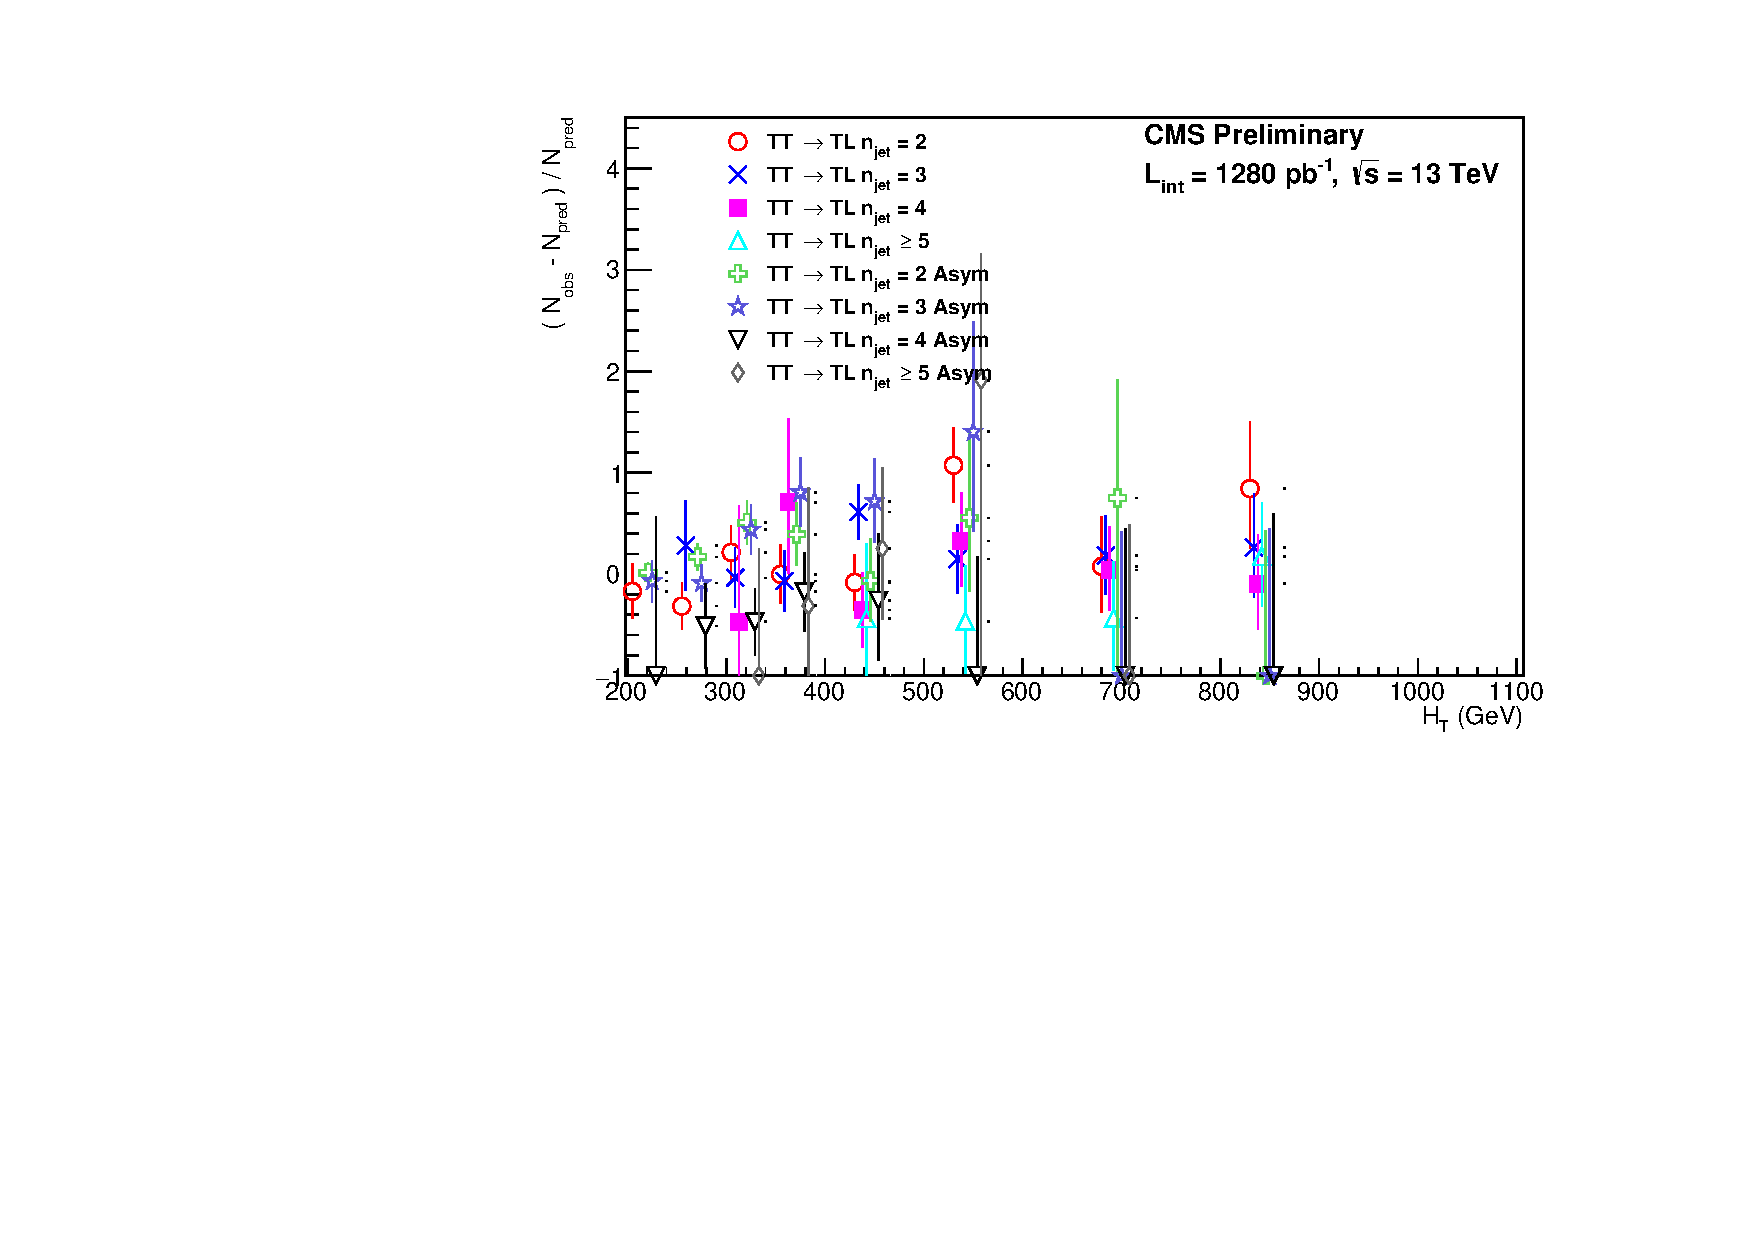
\includegraphics[width=0.6\textwidth]{figures/closureTests/newJamboree/looseLeptonCrossCheck.pdf}}
    ~~
    \subfigure[Pulls of closure
    tests]{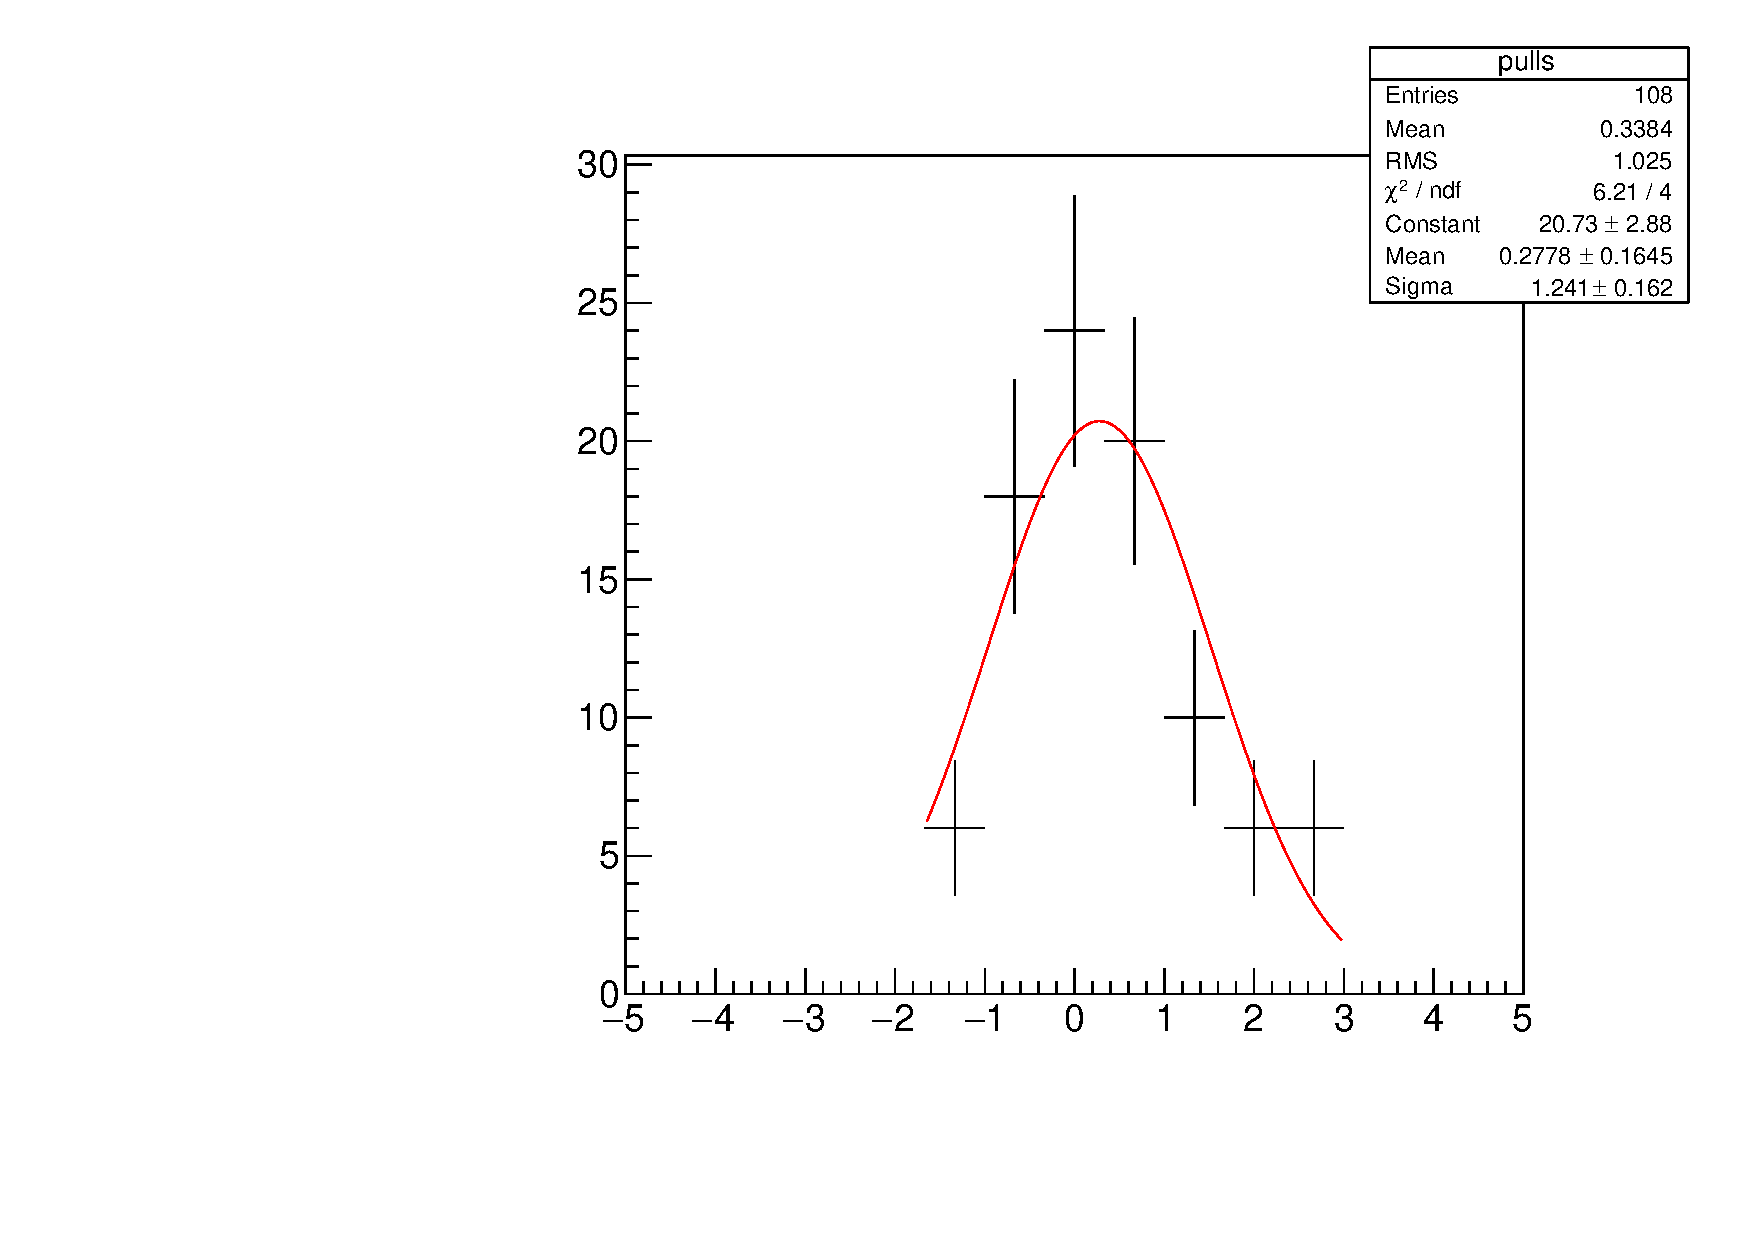
\includegraphics[width=0.4\textwidth]{figures/closureTests/newJamboree/looseLeptonPulls.pdf}} 
    \caption{Closure tests probing the effect of lost leptons in the
    analysis for each
    \njet category (open symbols) and their pulls fit with a gaussian.
    Carried out with $2.1\ifb$ of
      $13\tev$ data. Events with two muons that pass the control
      region (tight) muon criteria are used to predict events with one
      tight muon and one muon that passes the signal region veto
      criteria (loose)}
    \label{fig:closureLooseLep}
  \end{center} 
\end{figure}



